\section{Культурная и цивилизационная роль науки. Сциентизм и антисциентизм}

\subsection{Понятия «культура» и «цивилизация»: трактовки и взаимодействие}

Однозначной трактовки этих понятий не существует по следующим причинам. 
\begin{itemize}
    \item Данные категории по-разному понимают с точки
    зрения различных философских, исторических, социологических, культурологических
    Определение будет зависеть от оснований самого подхода/теории.
    \item Такие термины, как «культура и цивилизация» имеют более узкие и 
    более широкие трактовки (человеческой цивилизации вообще  
    или шумерская цивилизация; культуре вообще или европейская средневековая культура).
    \item Помимо общепринятого разделения понятий культура и цивилизация есть немалое
    множество немейнстримных классификаций, которые позволяют увидеть новые грани 
    в этих понятиях.
\end{itemize}

\begin{table}[H]
\centering
\renewcommand{\arraystretch}{1.5}
\begin{tabular}{|p{4cm}|p{4cm}|p{5cm}|}
\hline
\multicolumn{2}{|c|}{\textbf{РАЗЛИЧИЯ}} & \textbf{СХОДСТВА} \\ \hline
\textbf{Культура} & \textbf{Цивилизация} &
\multirow{5}{4cm}{\begin{itemize}
    \item Историчность изменений
    \item Человеческие феномены
    \item Классифицируют по социальным, моральным, политическим, экономическим, мировоззренческим, географическим и другим особенностям
\end{itemize}} \\ \cline{1-2}
Осмысленная \textbf{деятельность} человека и её продукты &
Совокупность материальных и духовных \textbf{достижений} общества в конкретный период \textbf{истории} & \\ \cline{1-2}
Совокупность \textbf{ценностей} человека (как духовных, так и
материальных) &
\textbf{Общность людей}, характеризующаяся специфическими чертами (соц. отношения, тип культуры, ист. и географ. рамки, эконом. и полит. ситуация) & \\ \cline{1-2}
\textbf{Образ жизни} (способ бытия) &
& \\ \cline{1-2}
\textbf{Знаковая} (символическая) система &
& \\ \hline
\end{tabular}
\label{table:culture_vs_civilization}
\end{table}

Главное интуитивно ощущаемое различие между терминами в том, что цивилизация --- это
какие-то люди, а культура --- что и как они делают.

Наиболее фундаментальное определение культуры: культура как способ бытия. 
Это универсальное, определение, которое подходит к самому широкому смыслу,
включающему не только человеческое бытие. 

% Когда говорят, например, культура
% микроорганизмов или культурные растения, имеется в виду и в какой-то
% определенный, специфический, по сравнению с иными, способ бытия. Что значит
% способ? Порядок организации тех или иных процессов, регулирующие нормы жизни,
% развития, деятельности, пусть и на генетическом уровне записаны они в языке.
% Структурность, определенная морфология, путь самоосуществления во всей возможной
% для себя полноте. И что касается человеческой культуры, она, собственно,
% человеческая, благодаря наполнению смыслом, пониманию этих порядков, норм,
% структур, организующих жизнедеятельность тем или иным способом. То есть все
% остальные определения из первой колонки укладываются в это, подразумеваются в
% человеческой культуре как в понимающем способе бытия, откуда интерпретация
% символов, осмысленная активность, наделение предметов и явлений ценностным
% статусом и так далее. Но здесь же очень важно понимать и то, что как
% человеческие существа мы в том числе природны, биологичны и наша культура не
% сводится только лишь к творчеству, хотя это ее, собственно, человеческое ядро.
% Очень многое воспроизводится, транслируется, воссоздается, копируется и так
% далее. То есть у нашей культуры есть продуктивный элемент, производящая часть, и
% репродуктивный уровень воспроизводства изобретенных форм. Этот механизм нужен
% для сохранения типа культуры, и мы огромное время в убеденных практиках
% воспроизводим нашу культуру. Конечно, собственно, человеческий уровень — это
% осмысленное воспроизведение, то есть все равно в уникальных единичных актах
% заново творения культуры. 

Аналогично, цивилизация --- это общество, исторически развивающееся в рамках определенной культуры, то есть действующее определенным способом на одних основаниях. 

% Мне кажется, что слово
% «общество» мы употребляем, когда говорим в том или ином историческом срезе,
% например, японское общество в период Эда или современное российское общество,
% которое, скажем, отличается от советского общества. Цивилизация же предполагает
% нечто более глобальное, длящееся в истории, сохраняющее базовые культурные
% основания на протяжении всей своей истории, к примеру, индийская цивилизация.
% Однако это один из вариантов трактовать соотношение культуры и цивилизации. А
% вот

\subsubsection{Cоотношение культуры и цивилизации}
Различные мыслители подмечают либо сходство и близость этих терминов, и
тогда отождествляют их, либо различия, на основании которых данные понятия
разграничиваются, вплоть до подчеркивания их противоположности. 

\paragraph{Отождествление понятий культуры и цивилизации.} 

Эти понятия понимаются в целом как совокупность знаний, верований, искусства,
моральных норм, законов, обычаев и т.д., имеющих место в том или ином
человеческом социуме. 

Представители: Эдвард Тайлор, М.К. Мамардашвили. 

В случае неразличения культуры и цивилизации, исследователи обычно
сконцентрированы на противопоставлении данных феноменов природе, имея в виду,
что человек, как культурное цивилизованное существо, поступает не только в согласии 
с природой, но развивает мораль и
общественные законы, которые не являются чисто природной необходимостью. 

Поэтому некоторые исследователи считают, что культура и цивилизация — вещи одного
порядка и, в принципе, указывают на одну и ту же специфику человека.

\paragraph{Противопоставление понятий культуры и цивилизации.}

Такая позиция встречается у немецкого философа Освальда Шпенглера. 

В своей известной книге «Закат Европы» он
проводит идею о том, что культура — это царство органически-жизненного, а
цивилизация — совокупность технико-механического. 

Жизненный цикл любой
культуры таков, что она постепенно развивается, на своем закате вырождается в
цивилизацию и погибает. 

Поначалу общество рождает артефакты своей культуры; со временем остаются только готовые техники и технологии, и люди без должного осмысления и творчества
продолжают по инерции ими пользоваться; жизнь от этого опустошается --- цивилизация разрушается, когда утрачиваются основание, духовность. 

\paragraph{Различение понятий культуры и цивилизации.}
Полагается, что культура определяет специфику типа цивилизации, лежит в
ее основе. 

Примеры:  
\begin{itemize}

\item \textit{Формационный подход в марксизме}

Карл Маркс, полагал, что у любой цивилизации одинаковый путь развития через
ряд общественно-экономических формаций:
первобытный строй, затем рабовладельческий, затем феодальный, затем капиталистический, 
в конце --- коммунистический. 

Маркс не отрицал видимого разнообразия культур,
однако, анализируя специфику исторических процессов, предположил, что в любом
обществе в контексте развития орудий труда и благодаря изменениям в типе
производства, экономических отношений, социальной иерархии имеют место такие
переходы. 

Перескочить какой-то этап нельзя, и особенности
цивилизации в текущий момент во многом обусловлены тем, на какой стадии
находится общество. 

\item \textit{Теория культуры П. Сорокина}

Питирим Сорокин сформулировал теорию культуры,
акцентируя внимание на том, что во
многом именно содержание ценностей определяет существо конкретно культуры. 

В развитии культур он выделял три стадии, определяющие тип цивилизации:
\begin{enumerate}
    \item Сначала в обществе доминируют религиозные представления.
    \item На переходном этапе они ценностно
    уравновешиваются с жизнью в материальном мире, объективной окружающей
    реальности (например, этим характеризуется эпоха Возрождения);
    \item Происходит перевес в сторону чувственного контакта с миром (например, как это произошло в Новое Время).
\end{enumerate}
Конечно, между собой культуры
отличаются и по экономическим, и по климатически-географическим, по этническим,
по исковым и так далее, другим особенностям. 

\item \textit{21 цивилизация в концепции Арнольда Тойнби}

Арнольд Тойнби предполагал, что на развитии цивилизации происходит по схеме
вызов, стимул, ответ. 

Каждое общество сталкивается с какими-то проблемами,
находит мотивацию и средства для их решения и формирует ответ,
противостоя этим трудностям. 

Далее на новом витке все повторяется. На каждом
этапе возможны стагнация или сбой, тогда цивилизация не способна дальше
развиваться и погибает. 

Так, исследователь на основании различных признаков
выделял 21 цивилизацию, среди которых и ныне существующие, и уже ушедшие в
прошлое (то есть не справившиеся на каком-то цикле своего развития с вызовами и
формулированием ответа на них). 
\end{itemize}


\subsection{Роль науки в культуре и для цивилизации}

Наука мыслится как один из видов культурной деятельности человека. 

Специфика науки и ее отношения к предметам своего изучения,
методология, ведущие способы познания влияют на культуру в целом, определяя
особенности цивилизации.

Формирующаяся культура накладывает на человека свой отпечаток, и его деятельность, в том числе научная, определяется нормами культуры.

\paragraph{Хосе Ортега-и-Гассет:} Человек — это всегда человек какой-то культуры или в рамках какой-то цивилизации. Мы поступаем определенным образом, потому что культура определяет нормы поведения, в ней уже даны идеалы и ценности. Поступая якобы по-новому, мы все же
действуем в горизонте нашей культуры.


\subsubsection{Пример: наука и культура в ходе становления эпохи Нового Времени в Западной Европе} 

Человек начал стараться максимально отличить себя от природы. 
В науке нормой стал эксперимент, мнение о том, что нужно над природой совершить какое-то насилие, чтобы  выпытывать у нее тайны. При этом в моде: парики, обилие различной косметики, маскирующие естественный вид человека; повальное увлечение механическими игрушками.

% Причем не хуже, чем в 15 веке тайны выпытывала из человека испанская
% инквизиция инструментами в предельно искусственном стесненном состоянии. Это
% мысль британского импирика Фрэнсиса Бэкона. 

С тем, чтобы подчеркнуть отличие человека от природы, наука изобретает способы
окрашивания тканей в яркие цвета, методы нанесения орнаментов, механизмы различных размеров и назначений. То есть наука обслуживает культуру и запросы общества, как в сфере развлечения, так
и в сфере производства. 


% Культурным и цивилизованным само собой принято называть нечто высшее,
% человеческое, высокое, духовное. Тогда получается, что раньше когда-то были
% нецивилизованные дикари, а потом люди стали цивилизованные, да и сегодня есть на
% земном шаре дикари, а есть цивилизованные, а еще надо почему-то, мы сами не
% знаем почему, но надо всех дикарей сделать цивилизованными, да? Вот искуда такая
% уверенность. Может быть, это не совсем верно, разве по-человечески есть разница
% между представителями первобытного племени и постиндустриального западного мира?
% И тот, и другой человек, и тот, и другой мыслит, что-то как-то оценивает в
% этических категориях, рассуждает, творит, а может быть разница в уровне развития
% всего лишь видимость, всего лишь западный миф, очередная схема, конструкция,
% которая для объяснения чего-то когда-то была придумана, но разве она везде будет
% работать? Просто может оказаться рядом человек другой культуры, который мыслит в
% рамках и под влиянием иных конструкций, созданных общественным мнением его
% социума, и вместо того, чтобы напрячься и попытаться понять его ход мысли,
% откуда что берется в его суждениях, нам легче отмахнуться, навесить на него
% ярлычок чужой, а уже поэтому автоматически плохой, некультурный, не
% цивилизованный. Подумайте на досуге, можно ли вообще ранжировать людей и
% общество по каким-то уровням? Возможно, закономерности везде одни, везде, где
% есть человек, есть культура и цивилизация, просто содержание различается, но не
% выше, ниже, не лучше, хуже, а просто одно, другое, третье. Многие годы я
% посвятила изучению различных культур через философские тексты, литературные
% произведения, общение с представителями из разных уголковых земного шара и могу
% сказать, что в каждой культуре есть находки, каждая по-своему ценна и очень
% важно так же, как в рамках своей культуры с другими людьми, знакомиться с
% другими культурами. Сквозь видимую внешнюю пестроту и непохожесть просвечивает
% всегда общечеловеческое и от каждого из нас зависит, принимать ли другого,
% обогащать ли свою душу, открываться ли новому навстречу, даже, казалось бы,
% совершенно непонятно.

\subsection{Сциентизм и антисциентизм}

В XIX веке в сознании западного человека прочно укрепляется мнение о том, что наука --- это благо, поскольку получение новых знаний позволило решить ряд насущных проблем и способствовало росту качества жизни. Такую мировоззренческую установку, согласно которой
ведущая роль в развитии культуры и общества принадлежат науке, принято называть \textbf{сциентизмом}. Представителями данной позиции являются позитивисты, в их числе Огюст Конт.

% Можно
% говорить в этом случае о культе науки как наивысшей ценности. Что касается ярких
% представителей данной позиции, науке приходят позитивисты и прежде всего Агюст
% Конт, французский мыслитель, основатель классического позитивизма. Само название
% этой концепции происходит от идеи науки как позитивного знания, то есть такого,
% которое приносит реальные плоды, ощутимые результаты, противоположность другим
% видам человеческой деятельности, которые либо слишком субъективны и эфемерны,
% либо догматичны, либо вообще больше запутывают, чем решают проблемы. 

Кризис классического естествознания, смена ведущей парадигмы в самой науке на рубеже XIX-XX веков, а затем ужасные события двух мировых войн XX столетия, когда научные достижения использовались во вред человечеству (химическое оружие, атомное оружие, эксперименты
нацистов над людьми) \textit{начали связываться} с последствиями бурного развития науки и техники, заставляли задуматься над позитивной ролью науки как основания человеческой культурности.
Такую мировоззренческую установку принято называть \textbf{антисциентизмом}.

% Ухудшение экологической ситуации на планете и появление других, так
% называемых, глобальных проблем человечества, гемографические перекосы,
% экономические кризисы, нехватка ресурсов и пищи, глобальной безопасности и так
% далее


% В
% результате вера в науку и ее возможности мягко говоря пошутнулась. Хотя, на мой
% взгляд, основной причиной переосмысления места и роли науки в XX веке все-таки
% послужила несостоятельность чисто научной картины мира, которая по определению
% просто не могла заместить с собой весь горизонт человеческой деятельности, как
% бы сильно нам этого не хотелось.

Антисциентизм может быть выражен в разной степени. Это спектр мнений: от сомнения в передовой
роли науки, до радикального отказа от научной деятельности и научного способа познания. 

\paragraph{Методологический анархизм Пола Фейерабенда.}
На многочисленных примерах показывает, что хотя методология науки выглядит правдоподобной и эпистемологически обоснованной, большинство крупных научных открытий делается вопреки ее
рекомендациям. Убедительность правил научной работы имеют скорее культурные и психологические корни. Т.о., руководство правилами и нормами в научном исследовании нецелесообразно.
Эти наблюдения ставят науку по в один ряд с другими феноменами культуры, которые также строятся не только на рациональных основаниях и тоже направлены на постижение мира.

\section{Специфика науки как вида культуры. Наука и другие виды культуры}

\subsection{Почему науку считают видом культуры?} 

В любом феномене действительности, содержится парадокс одновременного сосуществования противоположностей:
\begin{itemize}
    \item науку можно считать универсальным внекультурным феноменом (н-р, могут ли естественные
    науки, которые нацелены на изучение универсальных законов природы, различаться в зависимости от культуры).
    \item науку можно считать культурным феноменом (теории науки разных эпох могут отличаться как по содержанию формируемой картины мира, так и по способу ее построения)
\end{itemize}

% человеческой истории, общества? На первый
% взгляд, нет. Природа, как все то, что не создано человеком, одна. И
% закономерности, по которым она функционирует, соответственно, не человек ей
% задает. Человеку в этом плане доступно лишь познавать связи и регулярности и по
% своему усмотрению применять в своей практике. 
% Однако, не изменить
% фундаментальный порядок Вселенной, не установить собственные законы для не нами
% созданного мы не способны. что во времена первобытных людей, например, светило
% перемещались по небу по определенным повторяющимся траекториям, что в нашем
% современном мире ничего не поменялось. Даже перед взором сегодняшнего
% чрезвычайно развитого представителя постнодустриального общества небесные тела
% продолжают жить по тем же самым законам, что и несколько тысячелетий, за что там
% несколько миллионов, миллиардов лет назад. Кроме того, мы не раз уже
% возвращались к такой формулировке наука, как теория действительного феномен
% общечеловеческий, универсальный в том смысле, что выстраивать теорию, отражающую
% реальность, осмыслять теоретически может любой человек. А у нас вопрос уже
% заранее предполагает, что наука это обязательно культурно нагруженный феномен.

% Например, античные учения о
% первоматерии, а мы их понимаем, и более того, ими можем пользоваться для
% понимания чего-то в своей современной жизни, они нас могут вдохновлять на
% открытие сегодня. 

% Тем не менее, с другой стороны, это не означает того, что
% наука одновременно не способна быть и культурно обусловленным феноменом, и видом
% культуры вообще, в смысле, специфическим видом человеческой деятельности. Ну,
% как по 
% реально различаются в различных культурно-исторических локальностях. 

% Не только
% разные обозначения одного и того же могут возникать, как, скажем, римские и
% арабские цифры, но и разными путями идут науки. 
% Например, в то время, как в
% Древней Греции активно развивалась геометрия в Древней Индии алгебра. Все знают
% о том, что порох был изобретен в Китае как минимум за тысячу лет до того, как
% это было сделано в Европе и так далее. 

% Также статус науки по отношению к другим
% видам деятельности может быть разным в той или иной эпоху, в той или иной
% культуре. Поэтому нам нужно помнить здесь и о втором моменте. Та или иная
% трактовка зависит от угла зрения, от подхода с позиции, которого мы определяем
% базовые категории, в частности, науки и культуры, которые мы сейчас
% рассматриваем, как связаны или не связаны друг с другом. Наличие или отсутствие
% связи будет зависеть от определения, от тех условий, в которых мы рассматриваем
% науку и культуру. Поэтому мы должны, прежде всего, вернуться к нашим
% определениям культуры, чтобы увидеть науку как ее элемент, как вид культурной
% человеческой активности. 

% Так вот, если мы культуру, например, понимаем, как
% совокупность материальных духовных ценностей, формирующихся вследствие
% специфической человеческой деятельности, то, несомненно, наука может быть
% представлена как один из видов этой культурной деятельности. Если человеческая
% культура предельно широко понимается как способ человеческого бытия, то тем
% более наука движет тяга к пониманию, по знанию, собственно, человеческая
% активность, осмысляющая. 

Науку можно считать видом культуры по следующим причинам:
\begin{itemize}
    \item наука связана с постижением, осмыслением окружающей действительности и человека, осмыслением специфической человеческой деятельности;
    \item наука предполагает основания в виде идеалов, норм, правил организации
    научной деятельности;
    \item язык науки имеет символическое выражение и правила построения научных суждений;
    \item наука имеет цели и ценности, на которые ориентируются в своем развитии;
    \item наука порождает материальные и духовные продукты, полезные изобретения, а также теории и законы, помогающие человеку понимать мир, ориентироваться в нем.
\end{itemize}

\subsection{С чем сопоставлять науку как феномен культуры?}

Если мы понимаем культуру как совокупность норм,
традиций, символического выражения, принятых в определенном обществе, то к видам человеческой деятельности относится практически вся жизнедеятельность человека,
(за исключением чисто природных биологических процессов в нас). 

Продуктивнее считать, что человеческая культура базируется
на смыслополагающей деятельности человека, на таких практиках, в которых
происходит творчество смысла. Тогда можно выделить такие виды культурной человеческой деятельности: \textit{искусство, наука, философия и религия}.

% Но, когда человек готовит блюдо не
% просто ради еды, но, прежде всего, ради самого этого действия, приготовления,
% когда он в этой деятельности производит для себя смысл, что изобретает,
% исполняется в этом делании, блюдо становится произведением искусства, а его
% приготовление в таком случае можно назвать собственно культурной деятельностью,
% создающей нечто новое. Не потому, что такого блюда еще не было, но потому, что в
% данной совокупности обстоятельств человек весь собрался на этом приготовлении,
% только это творчество здесь сейчас для него есть. 

\paragraph{Почему не указан миф?} 

Миф в сравнении с остальными видами деятельности \textit{синкретичен}: содержательно в нем
слиты религиозные представления о сверхъестественном, нормы морали и права,
мировоззренческие ориентиры, и т.д. 

Миф своей смесью различных человеческих практик замещает собой полностью разветвление на
отдельные феномены культуры: в готовом мифе все объяснено. Т.о., мифы \textit{нерефлексивны}, в рамках их содержания нет возможности выйти к первопричинам.

\paragraph{Почему не указана идеология?} 

Идеология обычно включает описание устройства социальной жизни, взаимодействий в ней, регулирующей системы ценностей. Идеология не рефлексируется и ее содержнаие синкретично. 

\paragraph{Почему не указаны иные виды?} 

Педагогическую деятельность, право, спорт, технологии, производство и т.д. в пределе можно свести к одному из четырех базовых феноменов культуры философии, либо их комбинации.



% и самостоятельно думать, ставить его под сомнение не нужно,
% просто используешь, чтобы ориентироваться в мире. Например, вместо научных
% представлений обыденное сознание так и поступает, боится геномодифицированных
% продуктов, рассуждает о вреде прививок, верит в теорию всемирного заговора и
% нарисованных нейросетями птичек. 
% То есть , положения, безусловно,
% принимаются на веру. Содержание мифа работает до тех пор, пока не ставится под
% вопрос. Это означает, что после того, как миф сотворен, он уже используется лишь
% для воспроизведения культуры, но не в рамках смыслополадающей активности.




Что касается остальных видов
деятельности, мне хотелось бы показать вам, как можно в пределе , искусству, науки и
религии. 

% Поскольку слово искусство происходит от древнегреческого техно, имеющий
% смысл некоторого искусственного делания, обрабатывания, но потреблялась как для
% обозначения профессиональной деятельности, например, искусство врачевания,
% ораторское искусство, так и в плане изготовления предметов культуры, скажем,
% искусства кузнеца, гончарное искусство. Безусловно, для ремесла или современных
% масштабов производства необходимо, помимо практического мастерства, также знание
% закономерности, поэтому любые технологии можно трактовать как продукт совокупной
% деятельности науки и искусства. Спорт, пожалуй, можно отнести к видам искусства
% в том смысле, что спортивная деятельность обладает зрелищностью и нацелена на
% выражение красоты и способности человеческого тела. Педагогика может быть
% отнесена к науке, поскольку представляет собой систему знаний о методах и формах
% ведения образовательной деятельности, с другой стороны образовательный процесс,
% как деятельность научения, прежде всего осмыслению, есть философская работа,
% политика, как деятельность по управлению обществом, ориентирующаяся на то или
% иное понимание блага для всех членов общества или выделенной его части опирается
% прежде всего на этику, философскую дисциплину, осмысляющую категорию блага.
% Однако, безусловно, требуется и знание закономерности общественной жизни и
% искусства управления. Право также раздается из определенного понимания ценностей
% и поступков, то есть имеют эти как сиологические основания. Однако, важную роль
% играют и представления о духовности человека, о том, что является грехом, в
% какой степени требуют порицания, наказания и так далее. Это относится к сфере
% религии. Наконец, без знаний о специфике отношений в социуме, а также о логике и
% изложении осуждений не было бы внятной юридической системы. Таким образом,
% далее, обоснованным представляется сопоставлять науку с тремя равноправными
% феноменами культуры – философии, религии и искусства. Эти четыре вида собственно
% человеческой культуры выделяются еще и на основании того, что обнаруживаются в
% том или ином соотношении, встроенными в каждого из нас. Наука, философия,
% религия и искусство соответствуют четырем базовым компонентам человеческой
% осмысленности как таковой. Я знаю, я понимаю, я верю и я выражаю переживаемое.
% Друг без друга они не существуют, соединяясь в любом реальном человеческом
% существе, даже если человек занимается по профессии одним из видов культуры. Мы
% выбираем в качестве основной своей деятельности одну из этих сфер, поскольку
% чувствуем наибольшую склонность, наибольшую способность к одной из них, хотя,
% безусловно, от этого остальные компоненты нашего существа никуда не деваются.
% Более того, далее, если мы захотим, мы не сможем из себя их извлечь волевым
% усилием, решив, например, что раз я ученый, не могу перестать верить, скажем, в
% бога православной религии, однако нельзя перестать верить хоть во что-то, просто
% это место в нашей душе займет другой абсолют, сила природы или закон вселенной,
% та идеология, которая навязывается с экранов или в соцсетях, современное
% мифологическое осознание по поводу правильного образа жизни, все что угодно. Да
% и какое знание обходится без веры? В русском не случайно ведать, в смысле знать
% и исповедовать однокоренные слова, а с древнегреческого знания эпистема от
% пистис вера. Ну и, к примеру, есть такое представление о том, что атеизм
% соответствует как раз отсутствию в человеке религиозной составляющей, однако это
% неверно. Атеизм означает буквально безбожие отсутствие Бога на месте первой
% веры, но отнюдь не означает отсутствие веры вообще. Если бы мы по-настоящему ни
% во что не верили, мы бы шагу не могли ступить, поскольку не верили бы в то, что
% он получится. Просто зачастую мы не рефлексируем то, что вера у нас есть, хотя,
% видимо, поступаем мы благодаря ей в ее свете. Ни знания, ни понимания, ни
% переживания чувств невозможны без веры, как минимум без доверия к самим себе в
% плане, что знаем, понимаем, ощущаем именно мы. То же самое касается остальных
% составляющих нашей души. Например, люди говорят у меня нет художественных
% способностей. Однако, несмотря на то, что такой человек вряд ли исполнится как
% поэт, музыкант или живописец, творить смысл через произведения искусства может
% каждый. Ведь занимаясь наукой по профессии, мы слушаем музыку, смотрим кино,
% читаем художественную литературу, и в том числе через приобщение к этим
% произведениям творим для себя смысл, благодаря им что-то лучше понимаем
% собственной жизни, не ограничиваясь только лишь наукой. Или, с другой стороны,
% покажите мне хоть одно настоящее произведение искусства, которое было бы
% создано, например, без научных представлений об анатомии тела, сгонах физики,
% психологических особенностях восприятия, или без возникших благодаря науке
% цифровой обработки звука, графических редакторов, производства красок и так
% далее. Мираб Константинович Мамрадашвили об идее органов мышления или органов
% понимания, которого мы говорили в прошлой теме про социальный институт, актуален
% и в рамках текущего вопроса. В различной культурной деятельности люди изобретают
% или творят особые формы, благодаря которым становится возможным понимание. Этими
% формами или органами мышления могут выступать антологические категории
% философии, произведения искусства, научные теории, богословские интерпретации. И
% нет никаких препятствий к тому, чтобы этими нетелесными органами, как формами в
% изобретении которых каждый из нас соучаствует своими актами осмысления,
% пользовались для понимания различных аспектов в своей жизни разные люди,
% независимо от их профессии. Мамрадашвили приводит следующие примеры. Я вам
% сейчас процитирую объемный кусочек из его статьи «Нука и культура». Сикстинская
% Мадонна Рафаэля не культура, это произведение искусства, но оно, естественно,
% является и культурным объектом в той мере, в какой наше взаимоотношение с ним
% воспроизводит или впервые рождает в нас человеческие возможности, которых в нас
% не было до контакта с этой картиной, возможности видения, понимания и так далее.
% Видение и понимание чего-то в мире и в себе, а не самой этой картины. Картина в
% этом смысле не изобразительна, а конструктивна. Следовательно, рассмотрение
% культуры как собрание культурных ценностей, как своего рода предметов
% потребления для удовлетворения наших духовных потребностей, совершенно
% неадекватно природе этого феномена и не позволяет его описывать. Произведение
% всегда уникальный предмет, содержащийся в одном экземпляре, он неповторим и
% неизменен, он всегда остается самим собой, это то, что случилось однажды, и
% после чего возник мир Мадонны, в котором и мы продолжаем жить, но уже как
% культурные способные существа. Таким же культурным объектом является, например,
% закон ОМА, применяемый в электротехнике, но акт возникновения произведений
% искусства или продуктов научного творчества и их наличие в качестве культуры
% разные вещи, говорит Мадашвили. То есть, как картина, так и научный закон
% являются некими инструментами, которые люди творят, создают для понимания
% реальности. Обратитесь к личному опыту, бывает, посмотрев фильм, прочтя роман
% или узнав о научной теории, мы начинаем понимать что-то новое, важное. И
% практически каждый великий ученый не был только лишь ученым. Многие занимались
% музыкой, литературой, изобразительными искусствами, были последователями той или
% иной конфессии и философски осмысляли не только научную деятельность, но и
% человеческие проблемы, далеко выходящие за пределы профессии ученого. Взять хотя
% бы всем известных Альберта Эйнштейна, Вернера Гейзенберга, Илю Пригожина,
% почитайте их биографии и их труды по философскому осмыслению науки. 

\subsection[Взаимодействие науки и других видов культуры]{Взаимодействие науки и других видов культуры (миф, религия, искусство,
образование, идеология, философия и т.д.)}

\subsubsection{Наука и философия} 

\begin{figure}[H]
    \centering
    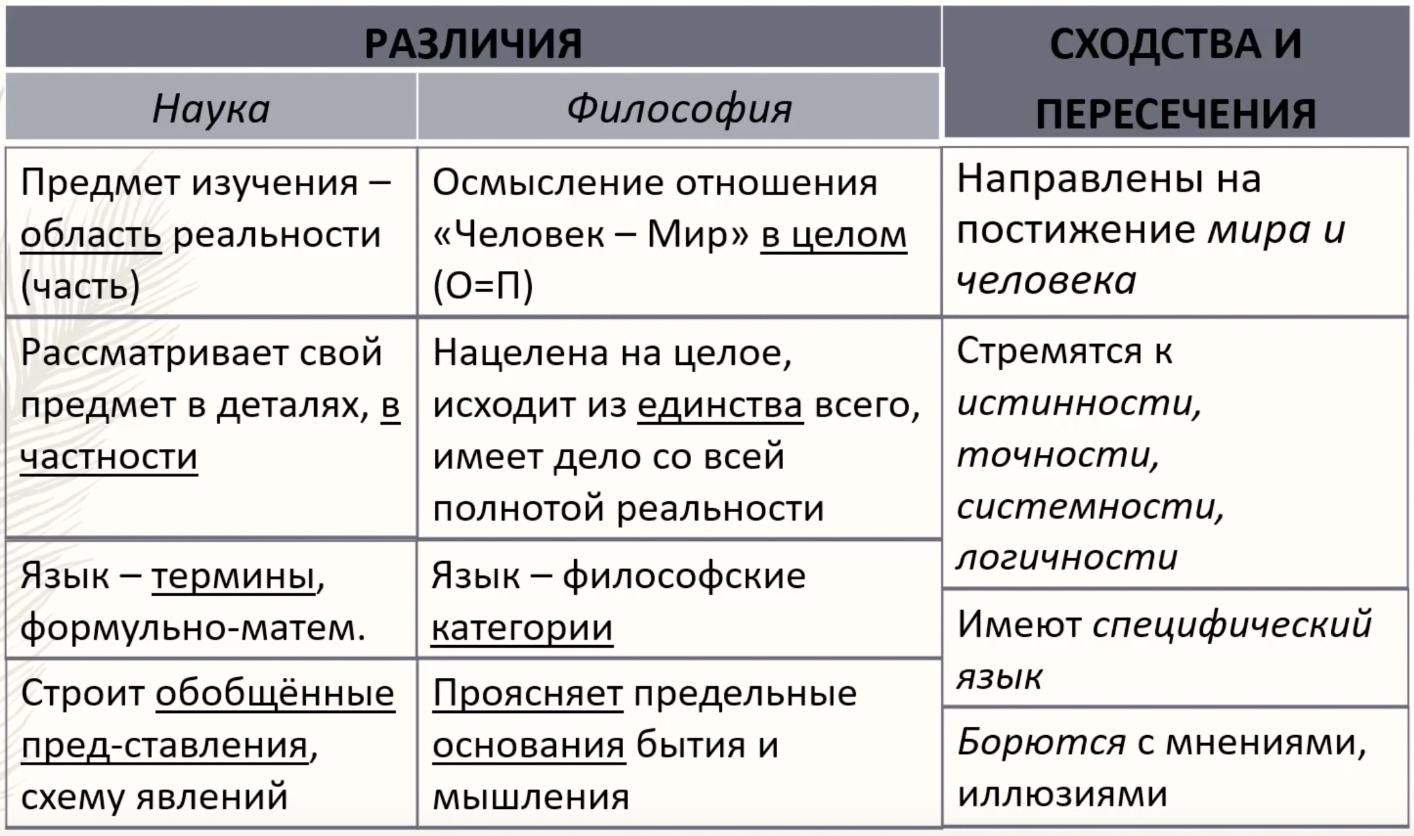
\includegraphics[width=0.8\linewidth]{pictures/sciphil.png}
    \label{sciphil}
\end{figure}

% Каждая наука выделяет в качестве предмета изучения определенную область реальности.
% Философия же занимается осмыслением отношения человек-мир в целом.  Сходство в том, что объект у этих видов культуры один --- действительность или то, что есть. 

% Философия нацелена на целое,
% в которое к тому же не только мир включается, но и мы сами во всей полноте и
% парадоксальности с плохим и хорошим и мира и нас. Поэтому объектом философии,
% который совпадает с предметом, является прежде всего отношение человек-мир в
% целом. 

% И различные философские концепции, а также настроенные в их свете
% умонастроения людей в различные культурно-исторические эпохи базируются именно
% на различном осмыслении этого отношения. Многие же, поскольку нацеливаются на
% формирование знания, вынуждены в свете этого целостного настроения вдаваться в
% подробности, детали, частности, то есть из всего в целом выделять для своего
% изучения предметы. Так в отличие от философии, представляющие в нас возможность
% и необходимость иметь дело с целым, каждая частная наука имеет в качестве
% предмета своего изучения какой-то кусочек реальности, какую-то часть целостного
% отношения человек-мир. Лингвистика язык, биология живую природу, химия состава
% превращения веществ, социология, человеческое общество и так далее. Наука по
% сравнению с философией избирает путь части, в том числе разбора на части,
% представления своего предмета как части реальности не в целостной слитости со
% всем остальным, а в его выделенности в частности. Несмотря на такие различия в
% нацеленности и философии и наука стремятся к истинности, точности, системности,
% логичности. Хотя требования, например, истинности суждения ученого-философа
% может пониматься несколько по-разному, невозможно себе представить, чтобы
% философские поиски и научные исследования ввели стремление к ложности. Здесь
% истина объединяет скорее даже не как эпистемологическая категория, но как
% этическая, поскольку выбор истины в противоположность лжи, прежде всего выбор в
% ту сторону, что мы считаем благом. Для своих различных задач, философии, как
% имение дела с целым, и науки, как познание аспектов реальности в частности, у
% данных видов человеческой деятельности, безусловно, имеются различные способы
% подхода к своим задачам и их решениям. Несмотря на то, что мыслительные операции
% мы производим как в науке, так и в философии одинаково, постановка, проблема,
% анализ, синтез, сопоставление, выделение общего и особенного, систематизация,
% формулирование выводов и так далее. Язык науки и философии различаются
% достаточно сильно. Каковы же языковые инструменты, используемые для выражения
% научной мысли, в отличие от философска. Этого мы касались в первом вопросе
% предыдущей темы, когда говорили о коммуникативных аспектах науки. Основы
% научного языка составляют особые понятия, которые называют терминами. Примеры мы
% тоже приводили, но давайте из разных наук еще повспоминаем вектор, рецептор,
% электроли, социальная группа, девиантное поведение, себестоимость, литерация и
% так далее. Помимо отсутствия в них экспрессивности, эмоционально ценностной
% окраски, первое, что также бросается в глаза, это точность терминов и
% стремящаяся к максимальной однозначности референтность, то есть строгое
% соответствие слова, словосочетания, наблюдаемому в реальности или так
% называемому идеализированному объекту, которым пользуется абстрактное научное
% мышление, например, материальная точка, абсолютно черное тело и так далее. В
% отличие от терминов в научном языке для философского основу составляют категории
% добро, красота, истина, свойства, структура, части целого, количество, качество,
% закон, уникальное, универсальное и многие подобные слова составляют несметный
% список философских понятий. Почему? Их нельзя поставить в один ряд с научными
% терминами. сделать это невозможно, как раз потому, что эти слова не имеют
% определенной референции в реальности, но задают сами условия нашей понимающей и
% исследующей работы с реальностью. Имеется в виду не то, что, не знаю, девиантное
% поведение, например, реально наблюдается, а красота или часть, нет. Речь о том,
% что у прекрасного и безобразного части и целого движения и покоя и так далее
% может быть совершенно различное смысловое наполнение, различное ценностное и
% этическое окрашивание в зависимости от тех мировоззренческих оснований в свете,
% которых мы называем нечто прекрасное, сопоставляем части целое, определяем в
% качестве движения или покоя. А, например, катет прямоугольного треугольника
% остается термином для его стороны, прилегающий к прямому углу со времен
% древнейших геометров и на протяжении истории науки свое значение не меняет. Мы к
% этому вернемся с вами сегодня в следующем вопросе и на примере категории части и
% целого рассмотрим, как их смысл различается в разные эпохи в зависимости от
% философских оснований каждой культурно-исторической локальности. Что же касается
% в этом плане сходств, несмотря на то, что в языковом плане наука и философия
% используют различные средства, объединяет их факт выражения своей мысли на
% особом языке, отличном от обыденного. Хотя философия во многом ближе к обыденной
% речи, чем наука, и всматриваться в естественный язык как в отражении оснований
% человеческого миропонимания, все же она с предельной строгостью говорит на языке
% понятий, которые в обыденной речи лишь интуитивно подразумеваются. Точнее, было
% бы сказать, что философия в этом плане имеет специальную цель разворачивание
% предельных смыслов понятий, в то время как обыденный язык их интуитивно как бы в
% свернутом, нераспакованном виде использует для цели коммуникации. И вот отличие
% языка науки от повседневного естественного языка еще более очевидно. На огромную
% долю наука в ее стремлении к установлению функциональных связей приходит в
% область искусственного языка, это прежде всего язык математики. Безусловно,
% обыденный язык, особенно в современности, в многом, благодаря СМИ, выхватывает
% научную лексику, вовлекая ее в коммуникацию. Однако, как и в случае с
% использованием философских понятий, от него не стоит ожидать строгого
% соответствия терминов их научным значением и глубокого четкого понимания сути
% явлений, так привлекательно умно названных наукой. И еще один пункт в нашей
% табличке давайте отметим, что мы имели в виду, когда определяли науку как теорию
% действительного. Тут предполагается ответ на два вопроса. с чем и как наука
% имеет дело, когда формируют знания. Наука имеет дело с предметами реальности. С
% беспредметностью наука не работает. Однако, то, что может в той или иной
% ситуации быть для человека совершенно не в предметном статусе, наука также
% способна делать предметы. Например, ощущение для художника, который его
% разворачивает в своей смыслополагающей деятельности, совершенно не то же самое
% ощущение, которое у этого художника наблюдает психолог. Для исследователя это
% предмет изучения, предмет психической реальности. А для художника этот один тот
% же феномен имеет значение не в качестве предмета, а в состоянии переживания, в
% котором он творит, и ему дела нет до того диагноза, который ставит ему психолог.
% И второй момент в нашем суждении то, что нереально науку не занимает. Даже
% виртуальная реальность, которой, на первый взгляд, в мире нет, на самом деле в
% какой-то мере реальность имеет место в нашей действительности и, надо сказать,
% немало на нашу актуальную реальность влияет. Поэтому к ней у науки информатики,
% кибернетики, психологии, социологии, математического моделирования и так далее
% проявляется не меньше интерес, чем, например, к природной действительности. А
% вот единорогам и русалкам ученые в реальности отказывают, поэтому, если ими и
% занимаются, то только как предметами фольклора или эстетическими образами
% филологии и науках об искусстве. Следующий вопрос, как наука со своими
% предметами имеет дело? Она их представляет, ставит перед собой. Как можно
% предмет научного исследования поставить перед собой? Не говоря уже о зрительно
% ненаблюдаемых для психолога феноменах психики или взаимодействующих молекулок у
% химика, даже медик, перед которым стоит человек, пациент, не может физически
% поставить перед собой человека вообще. Да, исследует тело он сейчас у
% конкретного человека, а у химика сейчас в колбе идет конкретная реакция. Но
% конкретными вещами ученые могут заниматься только в свете представления о
% человеческом теле вообще, о психике вообще, о химической реакции вообще. Наука
% не в первую очередь имеет дело с уникальным. На самом деле, каждый раз
% уникальным человеческим телом, психикой, животным, веществом и так далее. А с
% уникальным только как вариация воплощения универсального. Причем универсальное,
% общее, сходное, почему-то для науки важнее. Единичного, уникального,
% индивидуального. Между тем, как каждая конкретная вещь явилась ученому и самим
% исследователям, всегда прочерчивается экран обобщенного теоретического
% представления, которое абстрагирует или выделяет в уникальное, универсальное
% посредством наложения на уникальную, мыслимой, универсальной форму. Что же
% философия? Ее цель не составление знания о действительности, а прояснение
% предельных оснований бытия и мышления. И тофтологически, философия сама себе и
% цель и средство. Например, известнейший мыслитель XX века Мартин Хайдегер дает в
% своих лекциях такое определение «философия есть философствование». То есть,
% философия занимается осмыслением, пониманием, смысла всего в целом и продуктом.
% Такой деятельностью может быть только тоже мысль, понимание. Никакой другой цели
% у философии нет. Нет и никакого другого продукта. Это осмысление ради
% осмысления, собственно, человеческая деятельность. И если вам говорят, что
% философия имеет цель на первый взгляд нечто иное, например, научить чему-то или
% что-то воспитать, то имеется в виду научить мыслить или воспитать культуру
% мысли, но вовсе не научить жить, не научить какому-то мировоззрению, не научить
% мудрости. То есть, еще раз, главная задача философии не выдать какую-то
% информацию, а разработать и дать человеку инструменты осмысления, побудить его
% задаваться собственными вопросами и искать истину. Что же, в науке разве ученые
% не этим занимаются? В том-то и дело, как исследователи мы тоже осмысляем, но в
% рамках профессиональной деятельности ученого мы берем эти инструменты и в свете
% истины что-то видим, изучаем в своих объектах. А как философы мы как бы
% оглядываемся на то, благодаря чему есть то, что перед нами, на сам свет истины,
% который как бы у нас за спиной, когда мы познаем. Мы рефлексируем свою
% деятельность и даже если по профессии занимаемся наукой, это не значит, что в
% нас, как в живых человеческих существах, не присутствуют философские способности
% к видению мира в целом, постановки под вопрос даже устоявшегося знания и
% пониманию первопричин происходящего. Так вот, общее. Для философии науки мы
% уловили, должен рождаться смысл, должна присутствовать истина. Не только
% философия в своей, смыслопорождающей деятельности, борется с мнениями и
% иллюзиями. Науке не в меньшей степени приходится совершать усилия отделения
% научного знания от уже научного типа снежного человека, инопланетян,
% рептилоидов, экстрасенсов и так далее. Понятно, да? И объяснять в своих строгих
% формулировках научные законы в противоположность расхожим обыденным их
% трактовкам и неточным интерпретациям. Вы это, как ученые, прекрасно знаете по
% себе. Например, если мы скажем, что электроны вокруг ядра атома движутся по
% орбитам разной формы, сферическая, гантелеобразная или сложная в виде цветочка,
% химик или физик элементарных частиц нас поспешит поправить. Электроны, нельзя
% сказать, движутся вокруг ядра, тем более, конечно, не представляют собой эти
% орбиты. Объемные рисуночки, сферические, гантелеобразные, это условное
% изображение плотности вероятности наиболее вероятного пространства, опять же, в
% кавычках, нахождения электрона в том или ином энергетическом состоянии вблизи
% ядра. Не точка в пространстве с определенными координатами, а одновременно и
% волна, он как бы размазан по этой вероятной области. И вообще, давайте я вам
% покажу, откуда это все берется, обратимся к решению уравнения Шрюдингера для
% волновой функции. И понеслось. Ученые обязаны нас поправлять, возвращать из
% размытости обыденного представления на рельсы научного знания, иначе мы
% ориентироваться в мире будем по мнениям, то есть по мнимости, а не по точному,
% теоретическому. Философы по-своему борются против мнения, расхожих представлений
% и стереотипов. С их точки зрения, не специалисту простительно, например, иметь
% смутные представления об элементарных частицах, но непростительно, скажем, не
% рефлексировать навязываемые со стороны стереотипы о выборе профессии или о том,
% должно ли счастье быть общепринято. Но, в принципе, совершается сходное движение
% через объяснение, показывание ложности и губительности для нас таких
% недопроясненностей, готовых схем, удобных решений. 



\subsubsection{Наука и религия}

\begin{figure}[H]
    \centering
    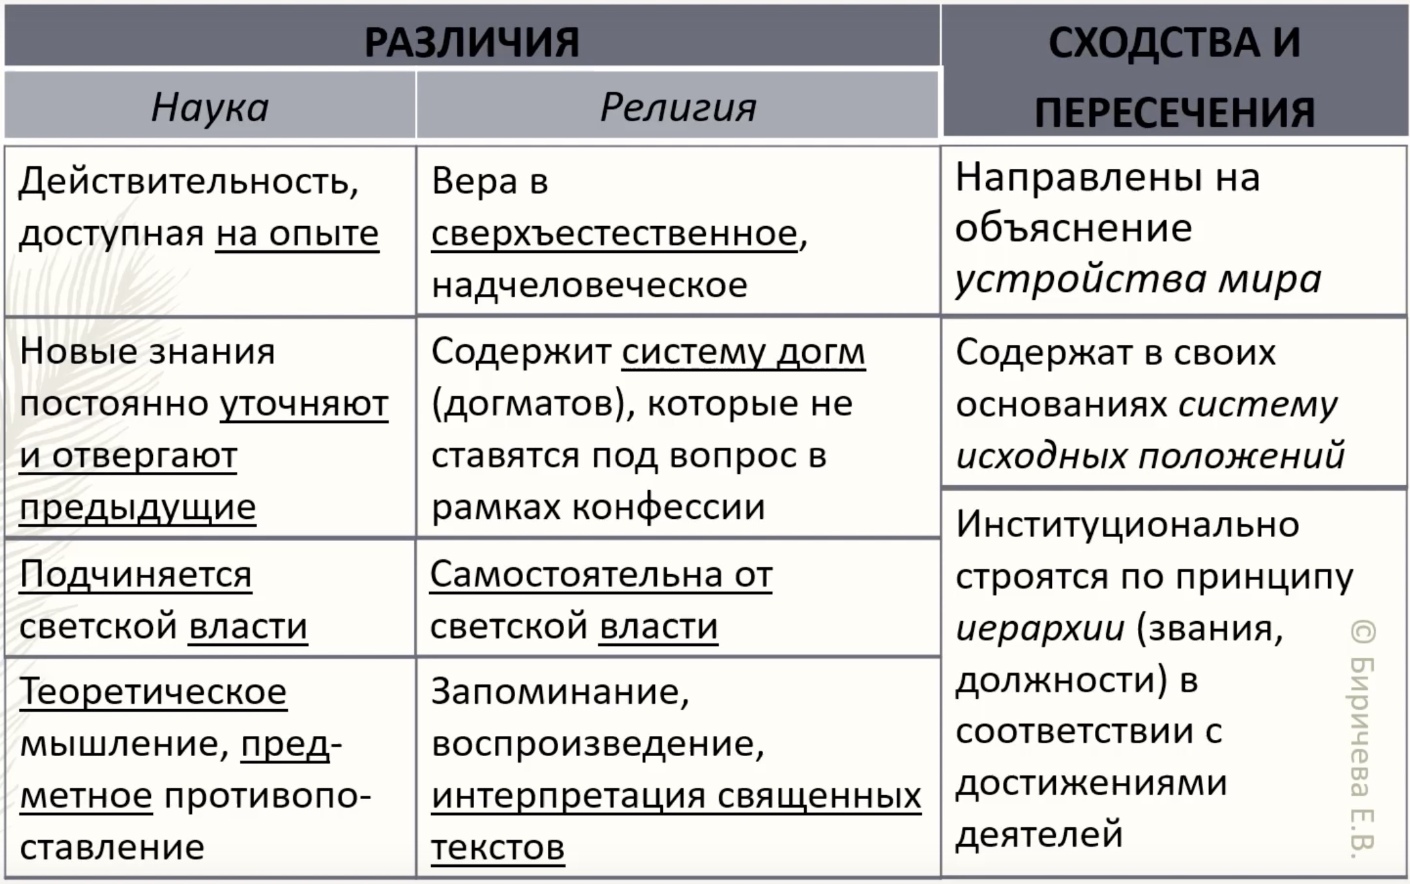
\includegraphics[width=0.8\linewidth]{pictures/scirel.png}
    \label{scirel}
\end{figure}

%  Прежде всего, отметим,
% что наука изучает объекты и явления действительности, которые доступны на опыте.
% Религия же основана на вере в сверхъестественное и трансцендентное, то есть
% антелеком посвящена незримым, высшим основаниям всего. А наука, как мы только
% что проговорили, сопоставляет с философией, имеет дело только с тем, что дно,
% что мы можем реально в мире встретить. Но, безусловно, оба эти вида культуры
% каждый по-своему объясняют первоосновы мира и трактуют как-то специфику
% человека, как внутримирного существа. Тут бегло заметим, чем религия отличается,
% в том числе, от мифологии, чтобы вы не путали. В мифе, конечно, есть
% представление о сверхъестественных силах, но, помимо этого, там намешаны и
% элементы других феноменов культуры, повествования о богах и героях, как
% эпические, литературные произведения, какие-то рецептурные рекомендации по
% поводу обустройства быта, философские концепции, так или иначе, трактующие
% благо, справедливость, природу, материя, способ возникновения мира, в жизни
% человека. Ну, понятно, да? Любая религиозная система концентрируется только на
% представлении надмирового, надчеловеческого, божественного, причем не
% обязательно бог один, не обязательно это сверхъестественное персонифицируется и
% не обязательно, кстати, божество вне мира мыслиться, то есть индуизм, даосизм,
% синтоизм и многие другие системы это тоже религии, а не мифологии, хотя, еще
% раз, может не быть антропоморфного божества, их может быть много и они могут
% мыслиться присутствующими в мире, а не вне его. Естественно, из этих
% представлений можно логически выводить какие-то этические рекомендации, советы
% по устройству быта, но это уже будут богословские, научные или философские
% интерпретации. Чего? Это второе главное отличие от мифологии священных текстов,
% которые содержат догмы или догматы, нерушимые и неотменимые в рамках
% соответствующей системы основоположения. Миф текуч, в нем возможны в самом
% разнообразные добавления, искажения, интерпретации при передаче из уст в уста.
% Любая конфессия фиксирует, свои базовые положения закрепляют священных текстов.
% И очень много усилий надо приложить, чтобы какой-то новый догмат ввести в эту
% систему. С огромным трудом подобное, например, удалось сделать в православии в
% XIV веке Григорию Паламе. Он предложил в противоположность католическому учению
% разделять понятия энергии и сущности в отношении Бога и его деяний. А вот
% скажем, такой шаг в сторону сближения с исламом, как иконоборчество, в
% православии в свое время потерпел неудачу. Вокруг этих ожесточенных споров
% творились поворотные исторические события, заключались под стражу и гибли люди.
% Так что религия четко держится своих догматов и немногочисленные случаи их
% изменения скорее исключения, чем правила. В отличие от этого, наука развивается
% путем постановки под вопрос действующих знаний и производства новых, уточняющих
% или преодолевающих предыдущие. Со второй темы можно здесь вспомнить
% постпозитивистов Карла Поппера и Тома Сакуна, которые по-разному предлагают
% рассматривать развитие науки эволюционно или путем научных революций. Но
% сходятся они в том, что все-таки со временем одни научные теории и подходы
% заменяются другими. Тем не менее, нельзя отрицать, что как наука, так и религия
% в любом случае содержат в своем основании систему исходных положений. Просто
% внуки они периодически пересматриваются, а в религии если пересматриваются, то
% возникает новая конфессия отдельно на своих основаниях и становится
% равноправными другими. Так, когда-то единое христианство разделилось на
% православие и католицизм, а затем от последнего отмежевался протестантизм в
% различных вариантах лютеранства, кальвинизма, англиканства и так далее. Об этом
% в темах о средневековье и возрождении вам подробно расскажет Светлана
% Викторовна. Какие еще отличия можно выделить? Обычно религия в современном мире
% существует автономно от власти, то есть давайте применять разобранные в
% предыдущей теме термины, институция анализируется в качестве самостоятельной по
% отношению к светской власти системы. А вот наука чаще всего входит в эту
% систему, подчиняется. Например, мы с вами на прошлой теме говорили, что
% Министерство науки и высшего образования РЭП занимается управлением и сельской
% деятельностью. Что касается в этом отношении сходств, институты науки и религии
% строятся по принципу иерархии должностей, званий, рангов, служителей или
% сотрудников в соответствии с достижениями каждого деятеля. То есть
% институционально предполагаются как в научном, так и в религиозном сообществах
% системы соподчинения и иерархического расположения в зависимости от тех или иных
% показателей, которые к тому же оцениваются специальными внутренними инстанциями.
% Наконец, в плане когнитивной специфики исследовательская работа предполагает
% теоретическое мышление, представляющее предметы в качестве противопоставленных
% знаний ученого. В религиозных практиках распространены в первую очередь
% запоминания, передача основ учения через религиозное обучение и интерпретация
% священных и авторитетных текстов. Также неотъемлемой составляющей являются
% строго регламентированные ритуалы, обряды, священодействия. В науке аналогом
% можно называть, пожалуй, соблюдение металлогических процедур, однако ввиду того,
% что они сами трансформируются, меняются, уточняются, изобретаются новые и так
% далее. Не факт, что это пойдет в рубрику сходства. Вообще наука и религия в
% современном мире достаточно полярные позиции, занимают по отношению друг к другу
% и трудно выделить много пересечений для них, глаза бросают скорее различия. Но
% думаю, того, что мы тут отметили, достаточно для представления экзаменей.

\subsubsection{Наука и искусство}

\begin{figure}[H]
    \centering
    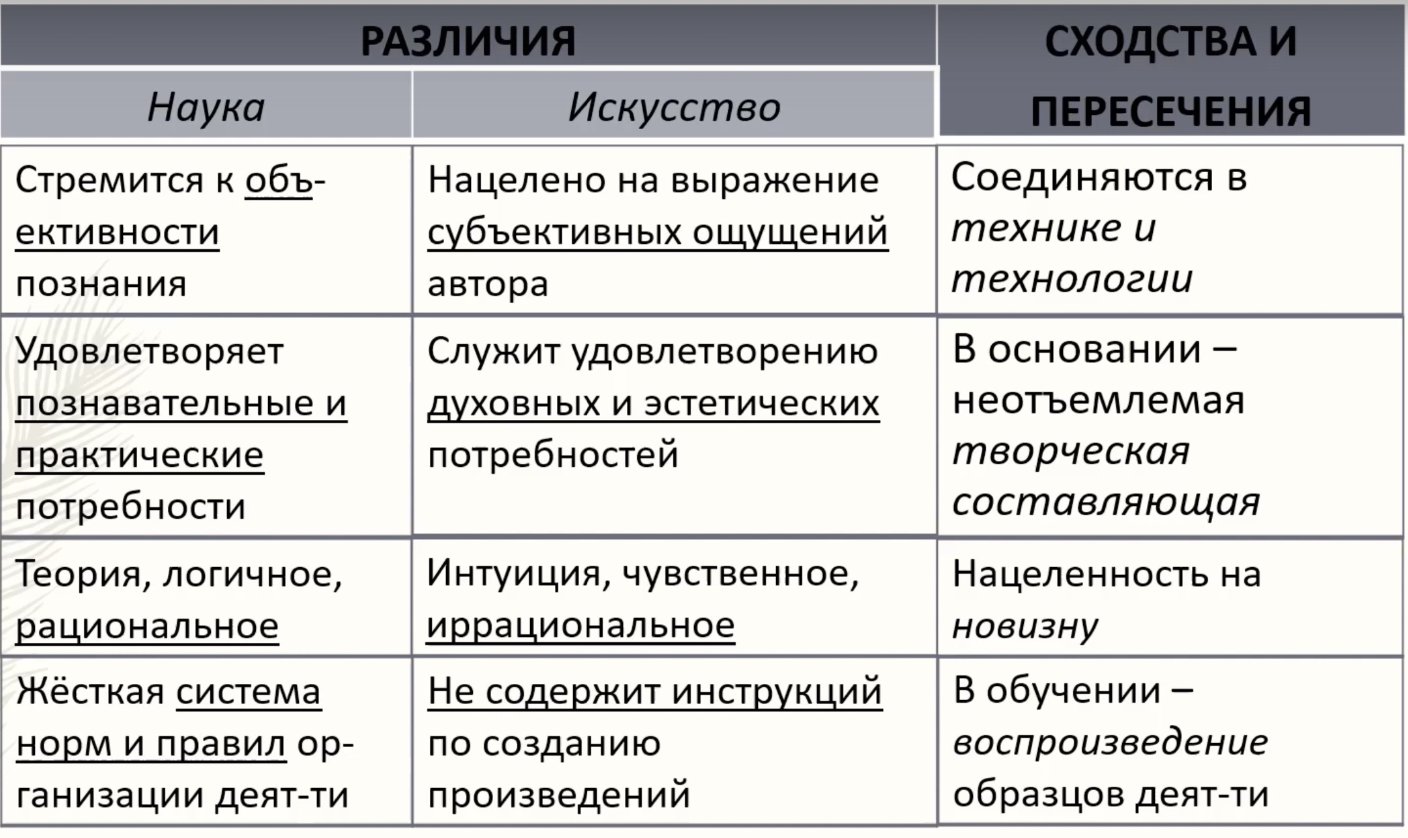
\includegraphics[width=0.8\linewidth]{pictures/sciart.png}
    \label{sciart}
\end{figure}

% поэтому перейдем к последнем сравнению, наука и искусство, чем у нас различаются
% и в чем сходятся. Тоже достаточно неблизкими друг другу кажутся эти виды
% культуры. Первое отличие, которое сразу приходит на ум, заключается в том, что
% наука стремится к объективности выражаемого знания. Тут объективность можно в
% двух смыслах брать, как отражение реальности самой по себе, представление его
% обобщенных законов и как противоположное субъективному, личному, то есть не то,
% что одному и не виду показалось, а что разделяется большинством в плане
% интерсубъективности. Искусство же не особо интересуется универсальными
% закономерностями и достоверным их описанием, а нацеливается на выражение
% субъективных переживаний и ощущений автора, его уникальной точки зрения, его
% новаторского способа видеть, пусть и ту же самую реальность. Пересекаются наука
% и искусство в технике и технологии. Это мы уже отметили, выше говоря, о
% древнегреческом слове техно, которое означает искусство в широком смысле как
% специфическая человеческая деятельность, направленная на создание того, что не
% рождается и не живет само по себе, но требует нашего осмысляющего участия. В то
% время, как наука направлено на удовлетворение мировоззренческих, познавательных
% и практических потребностей, искусство служит удовлетворению духовных и
% эстетических потребностей человека. Но и там, и там лежит в основании
% неотъемлемая творческая составляющая. Иногда кажется, что искусство это наиболее
% творческая деятельность, но на самом деле, во-первых, в искусстве огромную долю
% занимают те же самые коммуникации и рутинная работа, как и в науке, когда надо
% отточить мастерство, тренироваться, набить руку, много чего прочитать, обсудить
% с коллегами и так далее. А во-вторых, исследователь не менее творец, чем
% художник, просто он создает новое знание или техническое изобретение, а не
% картину или образ, скажем, спектакля. То есть, креативные способности можно в
% любой деятельности равно проявлять. При этом в науке мы опираемся на
% рациональные, логические, теоретические способности, а в искусстве большее
% значение имеет опора на интуитивные, чувственные и рациональные способности
% человека. Но, конечно, как и любая творческая деятельность наука и искусство,
% каждая по-своему нацелена на новизну. Наконец, можно такие еще различия
% предположить. Если наука имеет систему норм и правил ведения научного
% исследования, строгий язык, логику и так далее, то искусство не содержит
% однозначных инструкций по созданию произведений. Тем не менее, в обоих случаях
% обучение предполагает изучивание техник работы и задания на их практическое
% применение воспроизводства созданного ранее. Как, например, химику надо
% проделать множество лабораторных работ, воспроизводящих уже известные синтезы,
% аналитические процедуры и технологические процессы. Так и, скажем, скульптор
% сначала обучается слепить череп, вырезать барельеф, нагончарить кружку, а потом
% уже придумывает свой абсолютно новый шедевр. И далее, по подобной схеме вы
% самостоятельно на основе своих эрудиций и жизненного опыта сможете сопоставить
% науку с чем угодно, потренируйтесь на семинаре, это сделать по поводу
% образования, морали, политики и других феноменов культуры. 

\section[Культурно-исторический контекст развития науки и его философские основания]{Культурно-исторический контекст развития науки и его философские основания
(онтологические, гносеологические, этико-аксиологические)}

\subsection{!!! Понятие культуры в связи с её фундаментальными основаниями}

Культурология
знает, ведает, безусловно, чрезвычайно много о культурах, но сколько я не читала
труды исследователей в этой области, находила только поверхностные определения
культуры, не в смысле плохие, но замечающие только внешние проявления, все то,
что у нас обычно и ассоциируется с культурой, традицией и ценностями. Это все
замечательно. 

Однако, такое знание, хотя, несомненно, важно, интересно и для
определенных целей полезное, ничего не говорит о том, почему сложилась именно
такая культура, почему не другая, почему не иначе. Говорить, что так исторически
сложилось, или потому, что такой менталитет, или благодаря такому особому языку,
значит, повисать над бездной.
Мы всегда можем дальше спросить, а почему так
сложилось, почему такой язык и менталитет, на каком основании? 

Это только
философия может помочь, поскольку именно она занимается прояснением предельных
оснований человеческого бытия и мышления. И, по сути, понимание особости каждой
культуры делая ответы на тот же философский вопрос о своем собственном, которым
мы задавались на предыдущей теме, говоря об индивидуальном в человеке. 

Культуры отличаются своими традициями, идеалами, нормами, ценностями,
которые, в свою очередь, выросли из своего собственного, каждой культуры. Они
сформировались в свете определенного способа бытия, образа организации жизни.
Что значит способ бытия? это образ мысли, способ видения мира и себя в нем,
способ понимания окружающей действительности, в русле которого мы выстраиваем
свои отношения с миром, с природой, с другими людьми, с теми же продуктами,
имеющиеся культурой, в которой рождаемся. 
Поэтому мы и говорим, что философское
определение культуры это способ бытия, а именно в случае человеческой культуры
способ понимания человека мира и своего положения в нем, в свете которого
выстраивается определенное отношение к окружающей действительности,
результирующиеся в выработке норм и идеалов человеческой деятельности. 

Когда я
говорю об основаниях, как о способе бытия, я имею в виду, что оснований нет в
виде какого-то определенного что. Мы знаем, что исторически меняются содержание
научного знания, нормы и идеалы в искусстве появляются и уходят со сцены
религиозной системы и так далее. Надежное основание возможно только не
субстанциально в форме как образа действия или способа бытия. Конечно, плюрализм
или множественность оснований и в форме как, очевидно, в случае каждого
человека, но надежен для меня только мой способ бытия, другой не может быть за
меня моим способом, хотя с содержаниями мы можем с одинаковыми иметь дело.

Способ как конкретный путь, образ действий, по определению единичен, целостен и
уникален, то есть своей особостью и будет отличаться от других способов, но он
не зависит от того, на материале каких содержаний действует, он как-то поступает
со всем, что ему дано, что-то видит, что-то игнорирует, что-то использует, что-
то нет и так далее. На основании чего мы что-то делаем, видим, используем. Не
потому, что так принято или все вокруг считают это ценным. Мы можем поставить
это под вопрос и заменить одни говорят одно, другие другое, третье, третье. Кому
поверить? Почему надо вот это делать, не вот это? Что реально, а что иллюзорно?
Почему я к этому так отношусь? На подобные вопросы мы даем каждый пропускать
через себя, думавая по-своему, на материале, личностной истории и в свете своих
уникальных склонностей, способностей, наполняя смыслом, даем свои ответы. 

Мы
отталкиваемся от своего фундаментального основания, которое неизменное, а не
имеющимся из стороны в сторону, гонимые то одним, то другим чем-то мнением и не
слепо автоматически делаем, как принято. Иначе бы основания не переосмыслялись и
эпохи бы не менялись, и культура была бы у людей одна одинаковая по всему
земному шару. 

И вот точно так же, рефлексируя по направлению к основанию
культуры, мы приходим к необходимости прояснить самые фундаментальные из них,
то, в связи с чего мы мыслим и поступаем в бытии, речь об онтологических
основаниях, в контексте которых также возможным становится прояснение и других
философских оснований, гносеологических, этических, аксиологических и так
далее. Тогда, парадоксальным образом, философия у нас становится философией и
культурой, ведь именно прояснением этих оснований, понимания всего в целом, а у
разных культур они разные, мы занимаемся.

\begin{figure}[H]
    \centering
    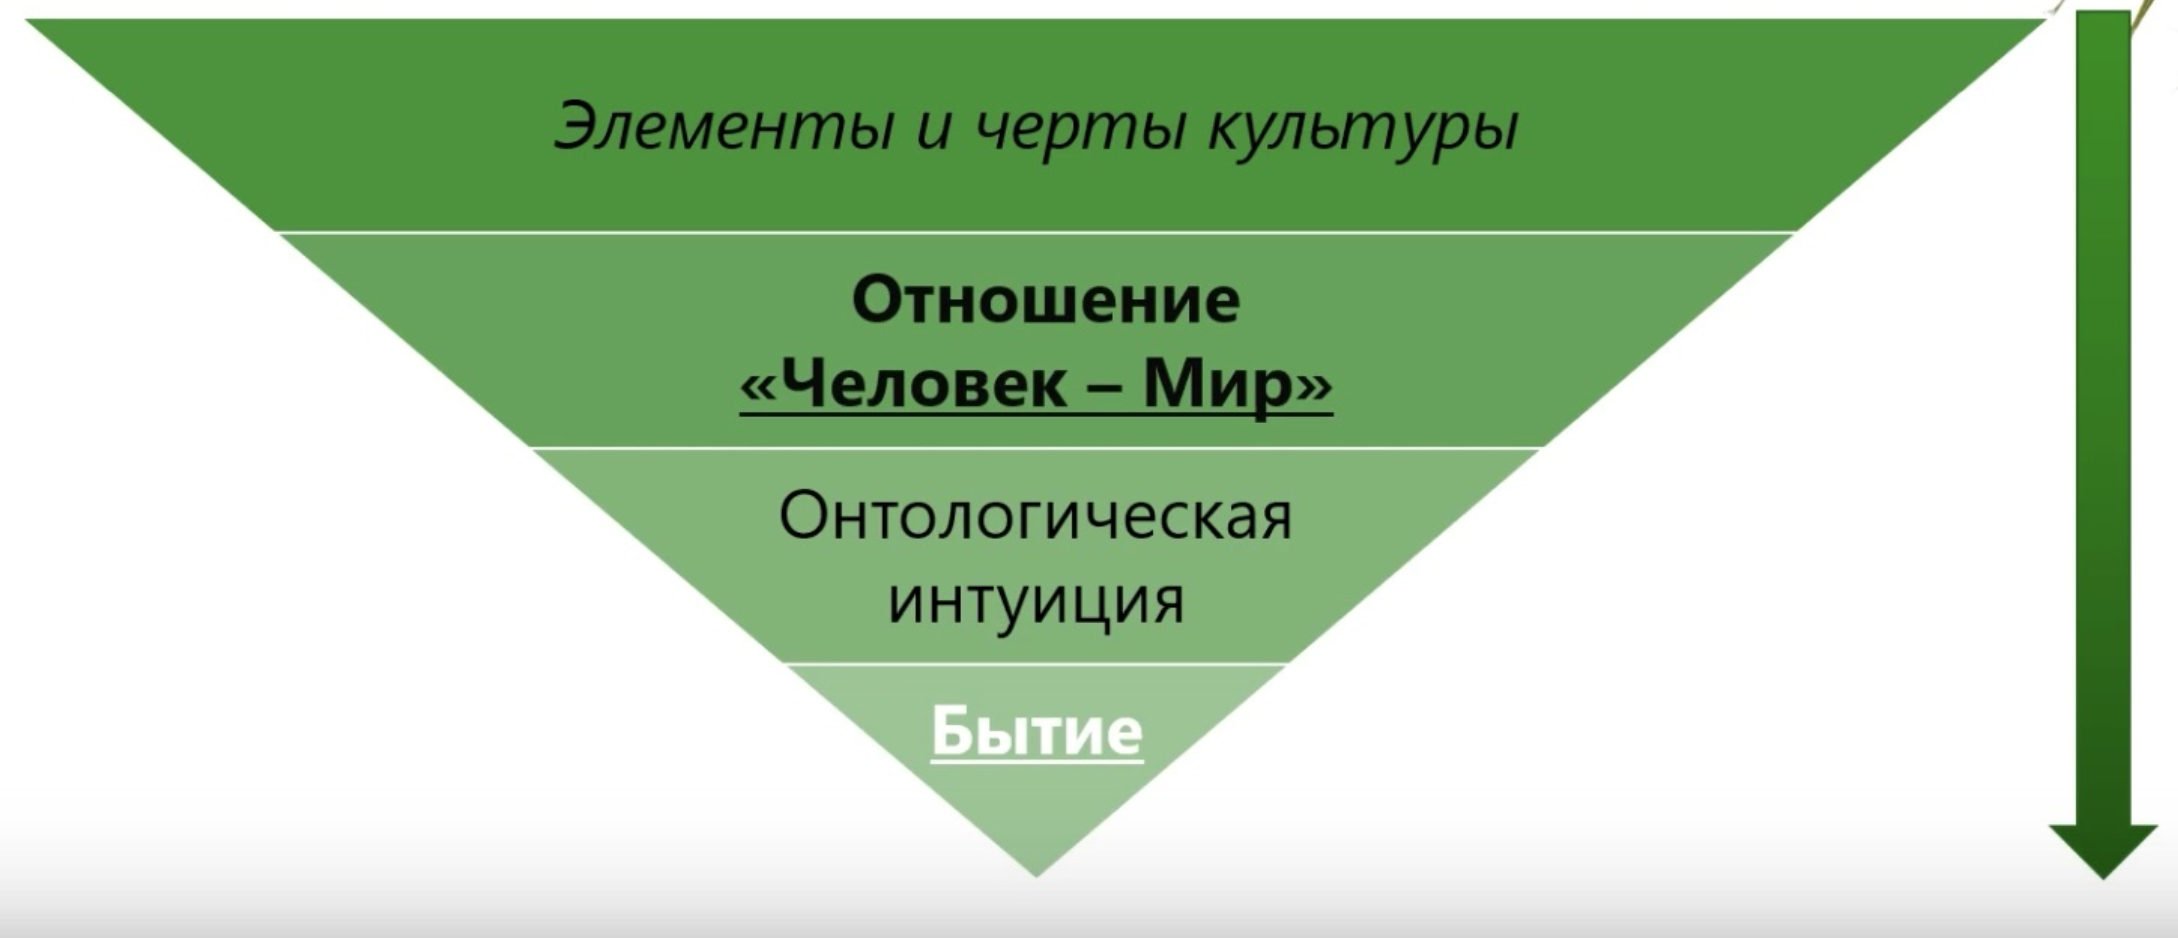
\includegraphics[width=0.8\linewidth]{pictures/hz.png}
    \label{hz}
\end{figure}

% В ротивоположность чему выстраивается способ бытия? причем каждый
% раз различный в исторической перспективе у представителей разных современных
% культур, в пределе у каждого человека.
% Бытие противоположно
% небытию и способ быть выстраивается вопреки или в ответ на страх небыть. То есть
% в основании нашего бытия предельным образом лежит на самом деле небытие,
% которого мы боимся, поскольку знаем о своей конечности и отталкиваясь от угрозы
% небытия стремимся быть максимально добротно быть, достигать пункты своего
% существования. Эту идею, причем применительно к осмыслению культурно-
% исторических трансформаций мировоззрения, проводит в своей книге «Муж что быть»
% выдающая немецкий мыслитель Пауль Тилли. тревога небытия постигается нами в
% глубоком детстве, обычно в возрасте от 3 до 5 лет, когда мы начинаем осознавать
% свою конечность во времени и пространстве. В пространстве мы познаем границы
% своего тела и то, что не можем по своему желанию непосредственно оборудовать
% другими людьми и внешними обстоятельствами. Безусловно, временность нашего
% существования каждым переживается как просто страх смерти. Однако, даже в языке
% есть такое выражение «Может быть что-то страшнее смерти». И вот для каждого
% человека в той совокупности окружающих его условий, в которой формируется его
% личность, то, что страшнее смерти, переживается уникальным образом и
% сворачивается с глубокого детства интуитивно в ту или иную форму угрозы небытия,
% чего, как вы думаете, можно бояться сильнее смерти. Например, хаоса и
% неупорядоченности, бессмысленности своего существования и окружающего мира,
% тотальной необеспеченности человеческого положения, возможности не оправдать
% ожидания окружающих людей, поступить не по совести, отказаться отделенным от
% всех, одиноким и так далее. Противоположность каждый раз конкретной форме угрозы
% небытия каждый человек выстраивает свой способ быть. Например, опасаясь хаоса,
% человек будет упорядочивать и рационализировать, структурировать и
% систематизировать все вокруг. Страх и необеспеченности логично развивать
% медицину и экономику, стараясь использовать природу на службу человека,
% удовлетворяя потребности и пытаясь продлить жизнь. Если человек боится не
% оправдать ожидания других людей, то посвятить себя благородному делу, вежливо и
% учтиво со всеми будет обходиться, учитывать интересы и особенности других людей,
% стараться соответствовать тем месту и роли, которые за ним закрепляются в
% социальной структуре и так далее. Тут, когда мы говорим о культуре, надо не
% забывать как раз о том, что культура как такой способ бытия не определяется
% географическими или национальными границами. Безусловно, языковая, социальная
% среда, историческая память, экономико-политическая ситуация связывают общность
% условий. Однако, это не детерминирует нас полностью, и мы можем принадлежать
% разным типам культур с ближайшим соседом, но почувствовать родство с человеком с
% другой половиной земного шара. Бредом, конечно, далеко не все люди осознают
% собственную тревогу небытия, да и кризисные моменты нашей жизни могут
% существенно повлиять на смену типа фундаментальной тревоги. В этом случае нам
% придется кардинально пересмотреть основания своих поступков, скорректировать
% характер, разменить жизненные цели и ценности. в графических регионах можно
% говорить лишь о преобладающем типе культуры. Наконец, последний момент,
% наверное, вы почувствовали культуру тревоги, хаоса и неупорядоченности, та, что
% исторически выросла на западноевропейской почве. Именно ее традицию внуки и
% философию мы, собственно, должны разбирать в нашем курсе. С ней заодно очень
% близко идет культура тревоги необеспеченности, как мне кажется, навязываемая
% сейчас ему миру со стороны США. В рамках глобализации сегодня мы, в смысле
% представители остальных культур, испытываем на себе влияние и, я бы даже
% сказала, давление со стороны этих двух типов культур, действующих совместно в
% плане стандартизации и универсализации, в том числе в сфере науки, в плане
% экономического расхода всего на планете, мечтания определения жизни, бессмертия,
% комфортного существования и подобных вещах. Это неплохо и нехорошо, просто важно
% понимать, откуда у современной науки ноги растут. Но важно не забывать, что в
% мире есть еще множество типов культур, в том числе наша тоже особенная. И нет,
% на ни хуже, ни лучше другой. Мы равноправны, поскольку каждый чувствует в той
% или иной форме экзистенциальную тревогу небытия и каким-то образом ей конкретно
% отвечают в своей ситуации, своим способом. способы не лучше и не хуже друг
% друга, потому что просто-напросто каждый хорош в отвечании на свою угрозу
% небытия и, понятное дело, плох, если им пытаться отвечать другому
% фундаментальному страху. В частности, поэтому на отечественной почве, как вы
% сплошь рядом видите, не проживаются решения, может быть, полезной и
% рациональной, но органично выросшей на почве иных культур. Таким образом, теперь
% мы в данной теме о культуре сможем заложить для себя фундамент понимания
% существа культурно-исторических эпох. Для этого опишем в логике культуры как
% способа бытия методологию, с помощью которой мы будем двигаться в темах
% следующего раздела, который называется «История науки в ее связи с философией»,
% начиная изучение каждого типа науки с прояснения его культурно-исторических
% условий и философских оснований соответствующей эпохи. Здесь также необходимо
% кратко привести конкретные примеры, какими были основания культурно-исторических
% эпох, которые нам предстоит изучать, чтобы стало хоть немного понятнее, как
% различное содержательное наполнение, ну, какое, да, наполнение могут получить
% основания и в соответствии с ними тип науки. Итак, антологические, сущностные и
% бытийные основания. Это фундамент определенного типа мышления, добираясь до
% которого сквозь все внешние наслоения, ну, там, традиции, социально-политические
% условия, ценностные ориентиры, мы как раз получаем ключ к пониманию оснований
% мышления, неважно, конкретного человека или культурно-исторической эпохи. Хотя у
% каждого из нас уникальное представление о себе, о мире и о своем месте в нем,
% если мы говорим о культурно-исторической эпохе, даже такой длительной, как,
% например, античность или средневековье, каждое существовало более тысячи лет, то
% имеют место тенденции примерно одинакового понимания этих базовых моментов всеми
% членами данного общества, сформировавшись в определенный момент, целостные
% представления о мире и человеке безусловно отражаются в языке соответствующей
% культуры, а с языком передаются в ходе воспитания от родителей и детям, то есть
% последующим поколениям. Поэтому смена культурно-исторических эпох происходит
% медленно, для с целыми столетиями. В связи с этим, например, так сложно провести
% разделительную черту между окончанием эпохи античности и началом средних веков.
% христианское мировоззрение, легшее в основу средневекового миропонимания, начало
% формироваться как минимум за четыре столетия до того, как оно получило тотальное
% распространение в Европе, сменив собой окончательно античный тип мышления. Так
% вот, сущностные основания того или иного типа мышления как раз предполагают
% определенное понимание отношения человек-мир, которое содержательно отличается
% для каждой эпохи. Одушевленная, упорядоченная, но при этом движущаяся,
% изменяющаяся вселенная античности с отражающим ее целостность и полноту
% человеком совершенно не совпадает со средневековым иерархически сотворенным по
% замыслу Бога миром, в котором человек уже чувствует себя иначе, в частности,
% например, не имеющим права на преобразование вещей мира, на буйную творческую
% активность и праздновать развлекательный образ жизни. Что касается бытийных
% оснований, естественно, во всей эпохе далеко не все люди настолько глубоко их
% для себя осмысляют и проговаривают, чтобы дойти до самой фундаментальной основы
% своего способа мысли, до понимания категории бытия. Категория бытия, то,
% благодаря чему все есть и есть именно так, представляет собой как бы пустую
% форму, наполнение которой в рамках каждого типа мышления также происходит по-
% разному. Однако нам в ободенной жизни достаточно интуитивного ее понимания,
% которое, опять же, в ходе воспитания нами усваивается. На этом основании мы
% сами, не задумываясь об этом, строим свои суждения и из этого основания выводим
% свои представления о действительности. На этом основании действия мы поступаем
% именно определенным образом. Прояснить и проговорить эти предельные основания
% всей нашей культуры, чтобы понимать, на чем все основывается, как раз задача
% философии и философов. Они занимаются профессионально глубокой рефлексией, то
% есть вопрошением о причинах, в пределе о первых причинах всего сущего,
% устройством мира, определенным способом мыслить и так далее. На самом деле все
% люди являются стихийными философами, поскольку периодически задаются вопросами о
% причинах стихийных событий, но большинство в силу посвящения себя иным занятиям
% не практикуют рефлексию настолько глубоко до бытийных оснований, особенно для
% нас исследователей это очень полезно для того, чтобы четко для себя понимать
% основания своих научных суждений и выводов теорий. Поэтому мы обучаемся
% философии и знакомимся с помощью ее метода с историей нуки. Так вот,
% антологическим основанием является помимо понимания отношений человек мир
% интуитивное понимание бытия. Здесь под интуицией имеется в виду не шестое
% чувство, а образ мысли, складывающийся в свете того, что остается для нас
% самопонятным, безусловным, несомненным, короче говоря, тем, что не ставится под
% вопрос. Это безусловный фундамент, от которого отталкивается любая наша мысль,
% то, что далее не может быть рефлексировано. Так, забегая вперед, для современной
% нашей эпохи, пожалуй, можно условно сформулировать антологическую интуицию, как
% интуицию сложного, множественного. Согласитесь, как в личной жизни, так и в
% своих научных исследованиях мы сегодня исходим из того, что все чудовищно сложно
% и многомерно. Кучу факторов нужно учесть разными методами, а не одним тестовать
% свои образцы, проследить многогранные связи друг с другом изучаемых объектов и
% явлений. Есть такое? Другой пример. Раз мы коснулись средневековья, в средние
% века несомненным было совершенно иное факт сотворенности мира Богом. Из этого в
% любом своем действии, суждении и понимании исходил западноевропейский
% средневековый человек. Это под вопрос не ставилось, иначе бы развалилось все
% средневековое мировоззрение. Наконец, самым главным антологическим основанием
% является понимание категории бытия в рамках данного мировоззрения. Понять
% антологическое существо эпохи определенного типа мышления означает понять ответ
% на вопрос, что значит быть для этой эпохи или в рамках этого мышления. Пример
% про средневековье быть значит быть сотворенным, быть на своем месте в
% соответствии с божественным замыслом. Тогда как для нас сегодняшних рискну
% предположить, быть означает нечто иное. Скорее всего в своей массе мы понимаем
% бытие как изменчивое, текучее, разнородное. То есть для нас быть скорее значит
% быть изменяющимся, трансформирующимся, развивающимся в сложной системе
% взаимоотношений с окружающей действительностью. Здесь конечно речь идет не
% только о том, что значит быть человеком, человеком в том числе, но в
% совокупности со всем сущим. Таким образом можно наш с вами метод исследования
% культурно-исторических эпох представить в форме условной схемы. Нам сейчас эта
% схема поможет как можно двигаться к антологическим основаниям культурно-
% исторической эпохи, чтобы понять ее существо. в начале стоит набросать контекст,
% разбираясь с действительными чертами и особенностями исследуемой культуры, то
% есть погрузиться во внешнюю специфику эпохи, в процесс чего можно будет
% прослеживать связи и закономерности развития этих особенных черт. Как при первом
% знакомстве с человеком, мы сначала воспринимаем его внешний вид, как он говорит
% и о чем, в какой манере, какие черты характера проявляет. На данном этапе
% знакомства с той иной культурой мы будем характеризовать как раз традиции и
% ценности в искусстве, в политическом устройстве, в быту и повседневной жизни
% людей, в социальных условиях человеческого бытия соответствующего периода. Более
% глубокая рефлексия далее выведет к антологическим основаниям эпохи, скрытым на
% глаз при поверхностном знакомстве, позволяя прояснить основную суть
% мировоззрения. Также с людьми, с кем мы начинаем понимать, почему человек именно
% так поступает в той или иной ситуации, почему у него сложился такой характер и
% на основании каких мировоззренческих принципов он высказывает те или иные
% суждения. То есть для культуры после краткого освещения контекста каждого
% исторического периода в рамках соответствующей темы, нам предстоит разобраться с
% тем, как все выделенные нами на первом этапе особенности сложились в свете
% определенного понимания отношения человек-мир. Здесь мы из принципов культуры
% будем выводить ответы на вопрос что такое мир представления данной эпохи, что
% такое человек и каким он должен быть, каковы место человека в мире. Далее мы
% сможем предельно почувствоваться в существо, рассматриваем культурно-
% исторической эпохи и постараемся улыбить антологическую интуицию, то,
% несомненно, из чего выводятся все принципы и особенности данного тип культуры.
% Наконец, мы придем к вопросу о том, что значило быть для того или иного типа
% мышления. То есть, дойдем до понимания категории бытия в том ее уникальном
% наполнении, свойственном именно конкретному варианту мировоззрения. Это, еще раз
% повторюсь, условная схема. Во-первых, можно исследовать эпоху или тип мышления
% другими способами, просто мы выбрали такой путь, позволяющий дойти до самой
% сути. Параллельно практикую усилия собственного осмысления, что тоже является
% важнейшей задачей для нашего курса. Во-вторых, конкретно эта схема нарисована в
% виде перевернутой пирамиды, однако это не значит, что бытие лежит в основании, в
% смысле какого-то квада, до которого нужно добраться. На самом деле, оно и без
% нашего исследования окружает и объемлет нас, дает нам быть, то есть не в смысле
% физического фундамента или какого-то ядра лежит у нас под ногами. Таким
% расположением слоев я хотела передать путь, которым наша мысль сможет двигаться
% по следующих темах при исследовании культурно-исторических эпох от поверхностных
% внешних особенностей к глубинной сущности. 

\subsection{!!! Система философских оснований и культурно--исторический контекст развития
науки}

Внешне система философских дисциплин может напоминать разделение науки на области знания. 
Однако разделы философии на самом деле не похожи на области исследований
в рамках науки, которые избирают каждое для себя какой-то пласт реальности и не
затрагивают другие. 

Каждая из них все равно имеет дело с отношением человек-мир, но смотрит на него сквозь призму
своих базовых категорий. Продуктивнее представить философию как кристалл, а ее различные разделы как грани. 
\begin{itemize}
    \item Онтология.
    
    Самая общая и фундаментальная грань. Онтология --- философская
    дисциплина, занимающаяся осмыслением бытийных и сущностных оснований отношения человек-мир. 
    Ее базовые категории бытие и сущие.
    
    Отсюда название греческие, то он означает то, что есть. Имеют относится
    пространство и время, качество и количество материю и идею движений, покой,
    части целой и множество других. Но все они получают свое содержательное
    наполнение в зависимости от того, как понимается бытие. 
    
    Или, если говорить
    проще, какой дается ответ на вопрос, что значит быть. Так что, говоря об
    онтологических основаниях определенной эпохи, мы сможем после прояснения самых
    фундаментальных перейти к разбору того, например, какие были представления о
    пространстве и времени или как понималась материя. 

    \item Гносеология.

    Область философии, занимающаяся вопросами познавательной
    деятельности сознания, проблемами сущности и видов знания, истинной
    достоверности сущности и методологии познания.

    То есть, гносеология тоже на все смотрит, но через призму категорий знания и познания. 

    \item Этика.
    
    Занимается пониманием блага в категориях добра, зла, долга, ответственности, греха и так
    далее. В рамках той или иной системы морали и нравственности. Базовая категория этики --- благо.

    \item Эстетика.

     Это философская дисциплина, осмысляющая сущность и формы прекрасного в художественном творчестве, в природе и в жизни. 

     Базовые категории --- красота, прекрасное.

     \item Антропология --- о человеке.
     \item Социальная философия --- об обществе и человеке как общественном существе
     \item Аксиология ---  о ценностях, идеалах и нормах.

     
\end{itemize}

% То есть, к примеру, гносиологию
% интересуют все о том, как мы познаем. Опознавать можно все, что угодно, от
% материала в руках гончара до природы блага, как такового, от букашки под ногами
% до Бога. Это все будут совершенно разные варианты познания, но все же познания.
% То же самое с эстетикой. Прекрасное, можно увидеть, услышать, ощутить во всем и
% выразить его в различных формах. Понятно, да? рамки, она высушенькая будет. Вот
% тут пример заполнения сразу. Далее. Самые фундаментальные антологические
% основания. Пропишите кратенькие ответы на вопросы. Как понимается отношение
% человек-мир, какова антологическая интуиция, то есть, что несомненно в данную
% эпоху и что значит быть или как понимается категория бытия. Мы обязательно с
% вами в таком ключе резюмируем базис античной культуры в следующей теме. У нас
% первый вопрос будет о социально-культурных условиях ее формирования. Из этого
% основополагающего ключа уже можно будет догадаться, даже если вдруг четко в
% лекции по какой-то эпохе вам это не проговорят, о ее гносеологических
% основаниях. Это какой основной источник познания, какие возникают и развиваются
% области знания, какие преобладают методы познания с этикой. Мы с вами уже
% знакомы по третьему вопросу прошлой темы. Здесь мы прежде всего спросим, что
% есть благо, как оно понимается, что такое хорошо, что такое плохо для каждой
% эпохи. Хотя это разные философские дисциплины, но вы понимаете наилучшее,
% наиглавнейшее, самое ценное моменты неразрывно связанные, поэтому тут же можно
% перетечь к аксиологическим основаниям, что ценится в соответствующую эпоху
% больше всего. какие существуют идеалы и нормы поведения, общения, социально-
% политической жизни и в том числе ведения научного исследования. Наконец, можете
% себе в последних двух колоночках помечать круг наиболее важных вопросов для
% представителей каждой культурно-исторической локальности и самих этих выдающихся
% деятелей эпохи, мыслителей и ученых. Так что, ребят, реально, эта полезная
% табличка, она будет содержать отмычку каждой теме. Тогда, если поймете несколько
% этих базовых философских оснований, выраженных в нескольких предложениях, ничего
% учить-то не придется, все об эпохе можно будет логически вывести из пары самых
% фундаментальных тезис. Сейчас глянем на примере. Мы уже выше об этом говорили,
% теперь давайте чуть глубже посмотрим, систематизируем и выведем из
% антологических все остальные основания для эпохи Средневековья. В антологических
% основаниях запишем следующее. Само по себе чистое бытие открывается в акте
% творения, которым Бог создает каждую вещь, причем сразу на ее месте с вложенным
% в нее замыслом. Так что быть в этой системе значит быть сотворенным. Кроме
% конечно самого Всевышнего, который и есть собственно чистое бытие, как говорили
% средневековые мыслители, для него сущность и существование тождественны. То есть
% он и есть само бытие творящее начало. Несомненным в таком миропонимании был как
% раз креационизм. Антологическая интуиция сотворенности всего. Под вопрос можно
% многое поставить, но вот то, что все создано дворцом, мыслилось очевидным. И от
% этого рефлексируемо или нет в своих действиях и рассуждениях отталкивался любой
% человек того времени. Поскольку Бог уже все задумал на своих местах, мир как бы
% эстетичен и иерархичен. Однако положение в нем человека странное. Он
% одновременно и тварь среди других вещей и живых существ мира, а с другой сам
% обладает творческими способностями. В этом он по образу и подобию Богу создан.
% Строится разветвленная иерархия мира от неодушевленных камней, от физических
% объектов до высших существ, ангелов, через растения, животные и человека.
% человек ниже ангелов в иерархии, потому что он имеет тело, а ангелы бестелесны и
% поэтому не могут совершать зло. Чем больше материального и при этом меньше
% самостоятельного движения, то есть меньше души, тем на более далекой от Бога
% ступени находятся сущие. Как из таких антологических оснований вывести все
% остальные основания и черты эпохи? Мы должны тут разглядеть фундаментальный
% парадокс. Для средневекового мышления он заключался в статичном и динамичном
% аспектах бытия. С одной стороны мир иерархичен, упорядочен, уже продуман творцом
% и все целиком в его замысле уже есть на своих местах. С другой стороны очевидны
% и само действие творения и динамика изменений в мире. При этом естественно для
% маленького человеческого умишки непостижимо как Бог творит. Тут и о ценностных
% основаниях параллельно можно отметить. Главное и первично это Бог, а самая
% чистая часть в нас душа, поэтому надо стремиться к спасению души, к праведной
% жизни. Проводниками в этом деле должны стать понимающие слово с большой буквы,
% зато кстати посредством чего Бог сотворил мир из ничего. Слово священного
% писания надо интерпретировать, объяснять простым людям. В этом основное обучение
% заключается, которое должно вести к праведной жизни, победе над грехами и
% спасению души после смерти тела. А например познание природы отходит на второй
% план в системе интересов средневекового человека. Но несмотря на то, что замысел
% творца и то, почему он все именно так организовал в мире непостижимо, познавать-
% то как-то тоже надо, хочется, тогда что будет основным источником познания?
% Тексты, слово священного писания и авторитетных источников, например, базовые
% диалоги Платона и некоторые труды Аристотеля, неоплатоников, а также первая
% интерпретация так называемых отцов церкви. Какие методы познания будут
% преобладать? Комментирование, интерпретирование текстов, из них выводилось все
% доступное о мире знания, в том числе о тварях и природных явлениях. В этом плане
% мы обязаны средневековью культурой цитирования научных текстов и разработкой
% приемов анализа и аргументации. Естественно, развиваться будут в такой системе
% прежде всего какие науки? Науки о слове, грамматика латинского языка, на котором
% общались и учились все средневековые исследователи, логика, риторика,
% герминевтика, искусство толкования, экзегеза и так далее. Вот мы с вами в двух
% словах, конечно, очень схематично и кратко, но зато достаточно точно схватили.
% Базовое основание такое непростое и далекое от нас эпохи. На эти основные
% положения уже накручиваете потом контекст, какие мы слизили, когда, какие
% вопросы обсуждали, почему для них те или иные проблемы выходили на первый план,
% казались более насущными. В конце концов, благодаря нашему кратенькому разбору,
% я уверена, у вас уже не возникнет желания верить каким-нибудь старым учебникам,
% утверждающим, что средние века это темное время, что науки не развивались в этот
% период, еще как развивались. Другое дело, что методами для нас сегодняшних
% непривычными и в основном это были не естественные науки, как мы бы сейчас
% сказали, а гуманитарные. Хотя и на соответствующей теме вам Светлана Викторовна
% об этом подробно расскажет, по-своему бурно и неоднозначно развивалась та же
% физика, но не путем эксперимента, а в рамках спора с настолько авторитетным
% автором, как Аристотель. Но не будем так далеко вперед забегать, все по порядку.
% Однако здесь я бело приведу вам еще один обещанный пример. Без таких понятий,
% как, скажем, части целая, невозможно будет никакая научная теория. Посмотрим,
% как от мировоззренческих оснований в той или иной эпохе зависит не только
% различное наполнение философских категорий, но и различие выводов для научного
% худомысля. Сравним представления о части и целом, которые складываются на почве
% античной и новоевропейской культуры. Для многих из нас сегодня очевидными
% кажутся классические новоевропейские представления о соотношении части и целого,
% соотносите со своим пониманием. Часть меньше целого, целое состоит из частей,
% часть не содержит всего целого, не отражает все целое. Целое делится на части,
% мельчайшие из которых элементарны. В неклассических и постнеклассических теориях
% мы как раз сталкиваемся с нарушением этих принципов, когда при распаде частиц
% части могут быть больше первоначального целого, или когда часть голограмма в
% свернутом виде содержит информацию обо всем изображении в целом. Но на каких
% основаниях мы можем о явлениях говорить в той или иной логике. Классическая
% механика нового времени строится на интуиции, если так можно выразиться,
% элементарного достоверного. Что это значит? Это значит, что сложное состоит из
% простого, что все можно разложить на части, из которых составлено целое. И если
% не понимаешь все в целом, разбери на части, как говорит Рене Декарт, части более
% маленькие, более простые, поэтому, поняв их элементарную достоверность, можно
% это все собрать, суммировать и поймешь целое. Таким декартовским правилом нас
% учили пользоваться еще в школе, мы им пользуемся нерефлексируемые, в том числе
% сейчас в науке, даже если уже на самом деле не классические объекты исследуем.
% Для античности характерна другая антологическая интуиция, то есть, несомненно,
% лежащая в основании всего, это единое с большой буквы. То есть, для среднего
% человека в античности несомненно было то, что все едино, что-то одно через все
% как бы течет, мир изначально целостен и един, и все выделяемые нами
% противоположности благодаря чему-то одному единому изначально вместе
% удерживаться, равновешиваться. Так вот, интересно, что часть в свете такого
% понимания не будет меньше целого и будет все целое в себе косвенно содержать или
% отражать. Любая часть, такая же единичность, как и целое. Это значит, что, во-
% первых, нет приоритета между частью и целым в том смысле, что и то, и другое
% важно. И то, и другое как бы одинаково воспринимают текущее через все единое
% проницаемо для него. Поэтому, во-вторых, в такой системе часть является
% модификацией целого, всего целого, единого, а не неполноценной представленности
% какого-то ограниченного набора свойств. Например, если мы от камня отколем
% кусок, то это вроде бы часть того бывшего целого камня, которое его меньше во
% всех отношениях. Но древние греки видят не так. Кусок большого камня тоже
% камень. В нем химические, геологические, метафизические свойства от
% первоначального целого не отличаются. Эта часть такой же носитель каменистости,
% как и первоначальный камень. А к тому же это материя как модификация единого
% первого вещества. Так что ничто не мешает этому куску камня со временем стать
% чем-то иным, перейти в раствор, например. То есть выразить иные возможности
% всего в целом. Нам так видеть непривычно. Чтобы так смотреть, так увидеть части
% целые, нужны другие глаза или вернее за спиной должен быть свет других
% оснований, в данном случае античной культуры, чтобы мы видели в свете единого, а
% не в свете сложного или сложенного, как мы сегодняшний привыкли. Так что и
% научные выводы, к примеру, о природе материи совершенно различны в античности и
% в новое время, хотя базовые категории, через которые определяются научные
% термины, сами слова одинаковы. Таким образом, становится ясно, почему мы так и
% заглавили первый пункт плана понятия культуры в связи с ее философскими
% основаниями. Понимание независимого существования культуры как способ бытия и,
% соответственно, каждой культурно-исторической эпохи будет невозможно без
% осмысления философских оснований, в свете которых существует культура.
% Современное привычное нам деление эпох, по крайней мере, европейских, основано
% на выделении исторических периодов, в рамках которых отношения человека в мир
% понималось в каждую эпоху определенным образом. Способ понимания мира, способ
% построения науки, жизненный вклад в каждую из этих эпох возникает не сам собой и
% не в силу социокультурных, культурно-исторических или каких-то подобных
% факторов, как это зачастую трактуют. Все эти факторы вторичны по отношению к
% пониманию устройства мира и места человека в нем. Так что условно можно
% представить себе наш сбор каждой эпохи в рамках как бы системы координат. Вот
% одна ось это хронологическое время и каждый исторический период у нас на ней
% локализуется по векам. На второй оси наши философские основания. Тут, конечно,
% любое сравнение хромает и мы не можем количественно их ранжировать, но отметим
% как некие блоки или пласты антологические, гоносиологические, отеческие и другие
% основания и черты эпохи. Наверное, ранжирование по степени удаленности от самого
% базового слоя антологии, которая как фундамент для дома необходима любой
% культуре. А культура, помните, да, способ бытия. Наконец, безусловно, эпохи
% внутри себя неоднородные и возникают какие-то ответвления или ракурсы видения
% базовых моментов и их трактовки. Это мы отметим на оси направления. Имеется в
% виду концептуальные различные подходы внутри одной эпохи. Так, в античности у
% нас будет многообразие натурфилософских школ, учения Платона и Аристотеля,
% эпикурейцы, стойки, неоплатоники. 
А в новое время будут рационалисты и эмпирики,
% материалисты и идеалисты, приверженцы релационной и субстанциальной трактовок
% пространства времени и так далее. Они такие разные, но все-таки они вместе
% принадлежат единому в своих самых фундаментальных основаниях способов бытия. Так
% что здесь мы запомним, что именно наше положение и мироощущение определяет
% жизненный уклад, культуру и специфику современной цивилизации, а не наоборот.
% Несомненно, и культура, в которой мы рождаемся, влияет на нас, представляя как
% бы первичную матрицу возможного отношения к миру. Однако, я говорю о тонком
% различии между принципами культуры и тем, благодаря чему эти принципы именно
% такие. Это различие культуры и ее оснований очень важно увидеть для того, чтобы
% понимать, почему и как происходит смена культурно-исторических эпох. Сама по
% себе культура как совокупность традиций, ценностей и принципов жесткой системы,
% которая должна быть устойчивой и неизменной, чтобы выстраивалось в нашей жизни
% что-то определенное. Но со временем эта жесткая структура, которая по
% определению не может в свою матрицу вместить все возможное отношение к миру,
% представляет собой лишь один из вариантов выстраивания этого отношения,
% перестает работать. Она как бы вырабатывает весь свой возможный потенциал для
% объяснения мира и перестает давать ответы на значимые вопросы в изменившихся
% условиях. Тогда и появляется необходимость переосмыслить основания культуры для
% того, чтобы выстроить новую систему, которая давала бы ответы на вопросы,
% интересующие человечество на данном этапе и вступить в новую эпоху как еще одну
% вариацию способа отвечения на вопрос о бытии. Словно, как мы уже отметили, эпохи
% не сменяются мгновенно, не бывает такого, чтобы человек заснул в одну эпоху и
% проснулся на утро уже в другую. Даже если в том числе сегодня мы чувствуем, что
% назрела необходимость основания культуры вновь переосмыслить, то своим волевым
% решением мы тоже не сможем повернуть колесо истории, постановив все, с
% завтрашнего дня начинаем жить по-новому. Это важно понимать. Эпохи
% трансформироваются одна в другую столетиями, поскольку только через несколько
% поколений накапливается критическая масса людей, мыслящих уже на новых по
% сравнению с предыдущими основаниями. Сосовские основания культуры поэтому
% определяют базовые принципы, в том числе и введение научной деятельности, то
% есть формируют способ научного познания сего специфическим для каждой культуры
% методами, нормами построения научных суждений, объектами и принципами
% исследования. В этом ключе и принято говорить о культурно-историческом контексте
% развития науки. Давайте вдумаемся в эту формулировку, что здесь подразумевается.
% Прежде всего то, что наука развивается. Это в свою очередь означает, что научное
% знание меняется. И тут важно проговорить два момента. Во-первых, то, что на
% смену одних концепций приходят другие, вовсе не значит, что меняется истина.
% Пока записываете по этому поводу, зачитаю вам кусочек из текста уже знакомого
% нам испанского мысли XX века ХС РТГ и Гассета. Возьмем, к примеру, закон
% семейного тяготения. В той мере, в какой этот закон является истиной, он,
% несомненно, был кею всегда. То есть, с тех пор, как существует материя,
% обладающая весом, существуют тела. Последние всегда вели себя в соответствии с
% его формулой. Тем не менее, пришлось дожидаться, пока в один прекрасный день
% XVII века его не откроет один человек с Британских островов. И наоборот, нет
% ничего невозможного в том, что в другой прекрасный день люди забудут этот закон.
% Не провернут или уточнят, поскольку мы предполагаем его полную истинность, а
% просто забудут и станут относиться к нему так же, как до Ньютона, не будут даже
% подозревать о нем. Это придает истинам двойное, весьма курьезное свойство. Сами
% по себе они предсуществуют всегда, не претерпевая ни малейшего искажения или
% изменения. Однако, то, что ими овладевает реальный субъект, подверженный
% воздействию времени, сообщает им видимость, историчность, они возникают в один
% прекрасный день и, быть может, улетучатся в другой. Ясно, что эта временность
% относится, собственно, не к ним, а к их присутствию в человеческом разуме. Во
% времени, на самом деле, происходит психический акт, в котором мы их мыслим. Он-
% то и является реальным происшествием, действительным изменением в череде
% мгновений. Строго говоря, история принадлежит лишь наше знание или незнание,
% говорит Артега Игаса в своих лекциях под названием «Что такое философия?» Таким
% образом, мыслитель обращает наше внимание на то, что наше видение той или иной
% истины зависит от типа культуры, в свете которого нам определенным образом
% открывается мир. До становления новоевропейской науки, до появления
% мировоззрения, определившего существо эпохи нового времени, тип мышления был
% таков, что необходимости сформулировать очевидное падение тел в качестве
% математически выраженного закона просто не возникало. Забегая вперед, приведу
% примечанием еще один пример, который мы с вами будем подробнее разбирать в
% исторической части нашего курса чуть позже. Мой любимчик, которого я постоянно
% цитирую, Вернант Гейзенберг, говорит о том, что неклассическая физика XX века в
% вопросе понимания материи на микроуровне возвращается к мысли Платона, который
% жил в V-IV веках до н.э. то есть это, с другой стороны, подтверждает то, что
% рассматривая развитие науки, нельзя теории прошлого считать неправильными или
% ненаучными. Они могут и не терять своей ценности, истинности, проницательности,
% просто кажутся нам другими, отличающимися от наших привычных в силу различия
% оснований, на которых они созданы, и языка, на котором они сформулированы. Эту
% идею глубочайшим образом в своем творчестве проводит еще один выдающийся ныне
% живущий отечественный философ Анатолий Валерийанович Ахутин. Анализируя
% различные отношения к природе в античности и в новое время, мыслитель
% показывает, что эти отношения соответствуют определенному опыту, форма которого
% задается пониманием категория бытия и некой фундаментальной интуиции, например,
% интуиция единого в античности. Неподготовленные взгляды могут показаться
% непонятными концепциями античных мыслителей, однако не стоит спешить и
% сомневаться в их истинности, логичности, правильности. Чтобы убедиться,
% правомерны ли выводы той или иной теории, нужно рассмотреть антологические
% основания, в свете которых она сотворена, а не судить ее по параметрам
% сегодняшней парадигмы. Например, обычно улыбку вызывают положение учения
% древнегреческих философов о первовеществе. Для них очень важно было понять, что
% собой представляет то, из чего все состоит. Учение представителя Милецкой школы
% философии Анна Ксимена, жившего в VI веке на нашей эре, говорится о том, что,
% цитируем Августина по аналогии мировой философии, «Анна Ксимен все причины вещей
% свел к беспредельному воздуху». И далее, и свидетельств других авторов,
% поскольку не все тексты философ Милецкой школы сохранились до наших дней.
% Движение же Анна Ксимен считает вечным, благодаря ему все вещи превращаются друг
% в друга, а различаются в воздух по своей плотности или разреженности своей
% сущности. При разрежении рождается огонь, а при сгущении ветер, затем туман,
% вода, земля, камень, а из этого возникает все прочее. Или Гераклит утверждал
% почему-то, что все состоит из огня, а Фолес думал, что из воды. Но, во-первых,
% не из огня, воды или воздуха в нашем сегодняшнем понимании, а из первого
% элемента стихии. А, во-вторых, для древних греков очень важно было понимание
% мира как единого. Все наши классификации и разделения вторичны. Мы их привносим
% для удобства, а на самом деле изначально все едино и состоит все из чего-то
% одного. Иначе не были бы возможны плавные изменения и взаимопревращение веществ.
% Мы не могли бы усваивать пищу, если бы она состояла из чего-то иного, чем мы и
% так далее. Так что в учении аноксимина, фолеса, гераклита и других этичных
% мыслителей все логично и соответствует античной интуиции единого. А в
% средневековом миропонимании что-то кардинально меняется настолько, что на
% занятии алхимией, то есть на превращение веществ, накладывается стражайший
% запрет. В то время, как в античной Греции, да что там в Египте на этапе четырех-
% шести тысяч лет до нашей эры, обычным делом было существение химических реакций
% и знание о них. Почему так происходит с химическим знанием? Потому что в
% основании средневекового типа мышления лежит интуиция креационизма,
% сотворенности всего Богом, причем, как мы выше разобрали, пример, каждая вещь
% мыслилась сотворенной в единичном уникальном акте творения. Иерархичность во
% всем тоже следствия того, что все Богом создано на своих местах. А значит, если
% человек попытается из одного вещества получить другое, он тем самым замахнется
% на преступление божественного закона, переделывание божественного замысла, как
% бы пойдет против воли Бога, который так уже все предусмотрел и ранжировал.
% Например, что свинец менее благородный металл, чем золото. Вот вам и развитие
% химической науки. Вещества не переставали превращаться, но их активное
% исследование в европейском средневековье приостановилось. Хотя нельзя и
% абсолютно ложное средневековое отношение к этим явлениям утверждать. Каждый
% химик, занимавшийся синтезом, знает, насколько уникально получаемое даже в сотый
% раз тем же способом вещество по мельчайшим примесям, влажности, дисперсности и
% так далее. Тот же единичный акт творения. Но, в отличие от Бога, мы творим не из
% ничего, а из определенных материалов. Таким же образом, например, геометрия
% эвклида не становится ложной после появления неэвклидовых геометрии. У нее свой
% набор определений и постулатов, положенных в основании. На основании других
% постулатов и других определений получается другая математика, описывающая
% пространство с другими свойствами. Однако, нельзя бросаться и в другую
% крайность, увидев самостоятельность оснований каждой исторической эпохи и
% отрицать преемственность исторически следующих друг за другом времен.
% Средневековая наука обязана своим существованием античной, не меньше, чем
% современная физика ньютоновской, то есть новоевропейском экспериментальном
% математическом естествознании. Здесь мы тоже упираемся в парадокс, а значит вот
% что-то очень важное, что запускает двигатель мысли. В связи с выявленным нами
% основанием различия культур получается, что с другой стороны несколько
% некорректно говорить о последовательном поступательном развитии науки, о ее
% прогрессии, хотя для нас автоматически привычно думать, что современные теории
% лучше, полнее и точнее теории прошлого. Еще раз подчеркну, различные
% антологические основания, поэтому нет лучше, хуже. Одни основания высвечивают
% один круг вопросов и подразумевают один набор методов их решения, другие
% основания смещают внимание к другим проблемам или даже скорее к несколько иным
% ракурсам постановки тех же вопросов и предлагают другие способы их решения. Тем
% не менее, различия оснований при этом не означают, что люди напряжены, бывают и
% перестают обращаться к другим исторически предшествующим типам мышления. То, что
% мы можем усваивать некоторые наработанные до нас других культурно-исторических
% эпох опыт и продуктивно использовать его в своем осмыслении, как раз позволяет
% провести непрерывную нить истории между нами сегодняшними и теми, кто уже для
% нас стал историей. И это также дает вдохновение на каждый раз новое. 

\begin{figure}[H]
    \centering
    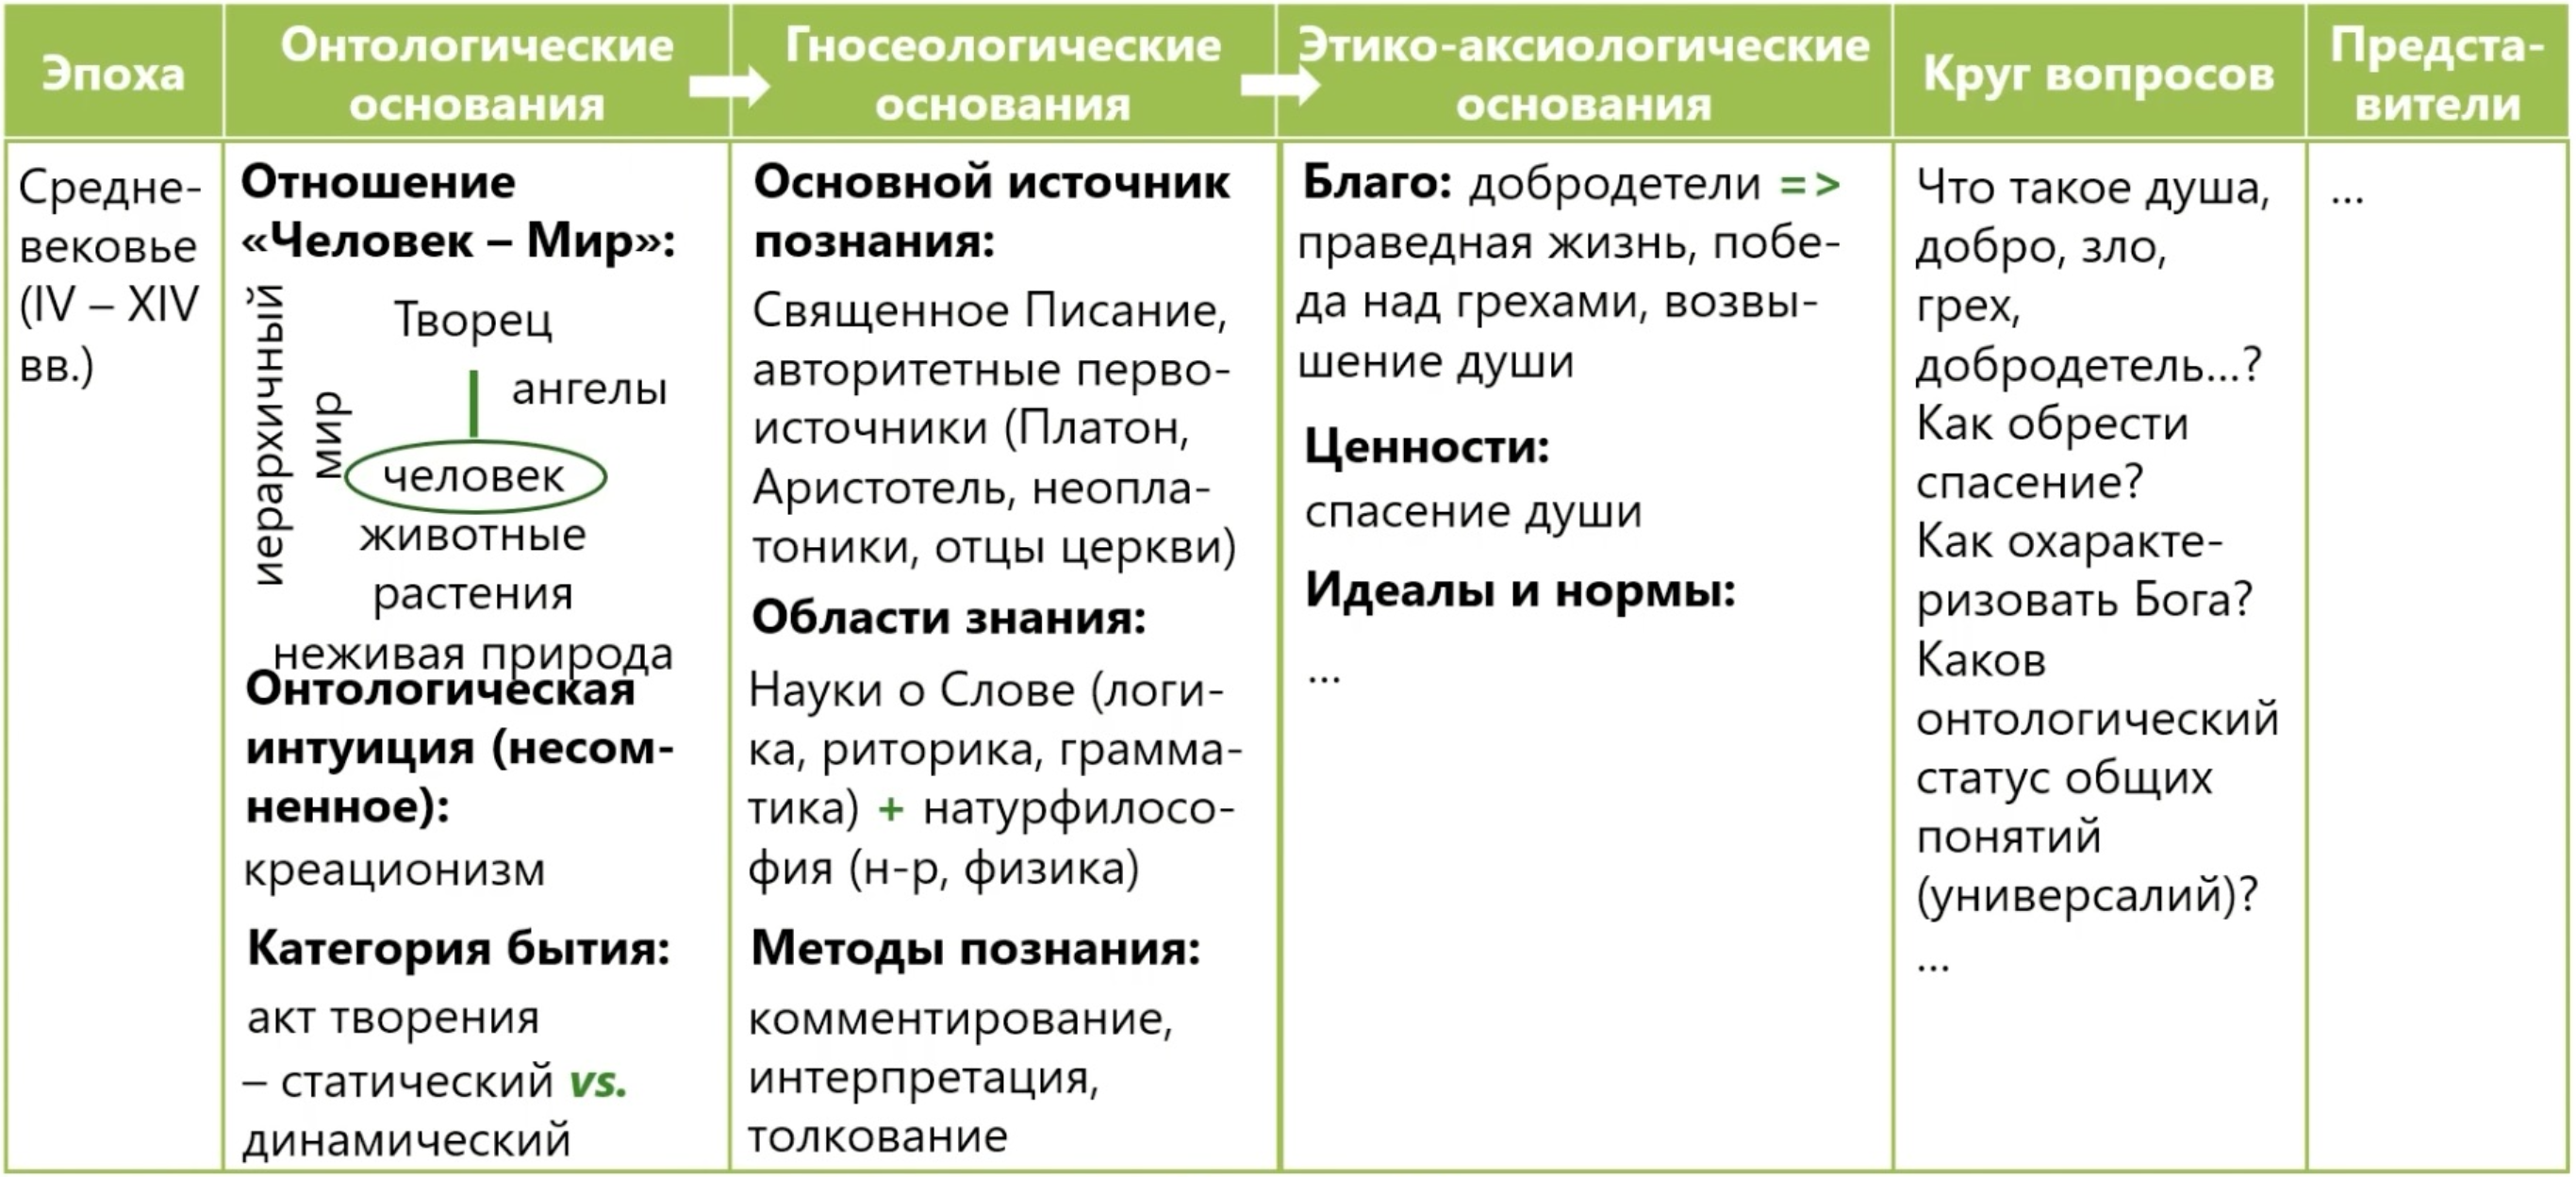
\includegraphics[width=0.8\linewidth]{pictures/med.png}
    \label{medieval}
\end{figure}

Гносеология изучает, как мы познаем. Познанию подлежит всё: от материалов до понятий вроде добра, от природы до Бога. Варианты познания различны, но это всё равно познание.

Эстетика интересуется прекрасным, которое можно увидеть, услышать, ощутить и выразить в разных формах.

Фундаментальные вопросы онтологии: как понимается отношение человек-мир, онтологическая интуиция, что такое бытие (В Средневековье: чистое бытие открывается в акте творения Богом, который создаёт каждую вещь; Бог — само бытие, сущность и существование тождественны; сотворённость мира Богом — очевидная истина.)

Мир Средневековья иерархичен: от неодушевленных камней до ангелов. Человек ниже ангелов, но обладает творческими способностями, будучи созданным по образу и подобию Бога. Мир эстетичен и статичен, но в нём есть динамика изменений.

Главная ценность Средневековья — Бог, а чистейшая часть человека — душа. Цель — спасение души, праведная жизнь. Основное обучение связано с интерпретацией Священного Писания и наставлением к праведной жизни. Познание природы второстепенно; преобладают методы комментирования текстов, авторитетными источниками служат труды Платона, Аристотеля, отцов церкви.

В Срнедневековье развиваются гуманитарные науки: грамматика, логика, риторика, герменевтика, экзегеза. Наука сосредоточена на слове; цитирование и аргументация становятся важными методами.

В античности мир воспринимался как единое целое, часть отражала целое. Например, кусок камня содержит свойства всего камня. В Новое время: целое состоит из частей, и части меньше целого. Декарт: понимание целого через анализ частей.

Каждая эпоха определяет культуру через философские основания. Отношение человека к миру влияет на жизненный уклад и способ познания. Эпохи трансформируются медленно, через накопление критической массы людей с новыми основаниями.

Наука развивается через смену концепций, но истина остаётся неизменной. Видение истины зависит от типа культуры (например, закон всемирного тяготения Ньютона --- истина существовала всегда, но была осознана лишь в XVII веке).

Понимание культуры невозможно без философских оснований. Исторические эпохи характеризуются различными способами познания, что связано с основными мировоззренческими принципами.

\subsection{Историческая проблема «начала» науки и деление на эпохи}

Задаваясь историческим вопросом <<в какой момент возникла наука?>>, прежде
необходимо определить, что понимается под наукой.

% с тем, на возникновение чего мы собираемся искать.
% Интересно, что философия науки, призванная заниматься осмыслением феномена науки
% в его бытийной и познавательной укорененности относительно молодая область
% исследований, начала выделяться в самостоятельную дисциплину, она лишь во второй
% половине XIX века с остановлением позитивизма, а прочное место в ряду
% университетских курсов заняла девушка к середине XX столетия. Такое позднее
% формирование отдельной философской области, посвященное специальному
% исследованию науки, наводит на мысль о недавнем по сравнению с искусством,
% религией, философией возникновении самой науки как специфического феномена,
% привлекающего к себе внимание лишь с недавних пор. 

% Задаваясь вопросом о том,
% когда наука стала такой, какой мы ее сегодня видим, с ее математизацией,
% экспериментальностью, небывалым размахом в плане масштабов внедрения во все
% сферы жизни и деятельности человека, 

Понимая науку как экспериментально-математический способ рационального познания мира, 
мы неизбежно упираемся в основание новоевропейской науки (рубеж XVI-XVII веков). 

% И достаточно распространена в современных исследованиях
% позиция, согласно которой науку считают самостоятельным видом деятельности,
% начиная с рубежа , в силу установления математики в качестве
% фундаментального языка описания природы и эксперимента в качестве ведущего
% метода познания. 
% В результате, отталкиваясь от данных, основополагающих
% концепции, большинство философов науки XX-го столетия обосновывает ,
% то есть науки в новоевропейском смысле. Этот смысл имеет и английская science.
% Как указывают исследователи, с одной стороны, до Галилея и Бекона не
% существовало экспериментов в собственном смысле слова, а с другой, наука,
% предполагающая царство рациональности, становится методологически строгой и
% математически точной, начиная с философии Декарта, положившей именно разум и
% рационально-логические законы пользования им в основании отношения человека к
% мир. Однако, понимание науки как феномена берущего начало в Европе в новое время
% и развернувшегося в XIX-XX веках в тот социальный институт, который сегодня
% повсеместно господствует, ставит обоснованный вопрос о европоцентризме или
% западном происхождении науки как таковой. Представители иных культур, в
% частности мусульманской, вполне закономерно возражают, что те неотъемлемые
% элементы, за которыми современная западная культура склонна видеть свое
% первенство, возникли задолго до XVII века в различных культурно-исторических
% локальностях. Так, например, математика с счетом геометрическими формами,
% которые одинаково для любого сознания человек пользовался по всей видимости
% столько, сколько существует человечество. В Древнем Египте и Мисопотами за 6-4
% тысяч лет до нашей эры на высоком уровне Личили, к примеру, было известно
% процедирование зубов. Были развиты математика, астрономия, фармацевтика, химия,
% сельскохозяйственная наука. В Древнем Китае, помимо остальных известных
% достижений, порох был изобретен не без экспериментирования, как минимум за
% тысячелетия до того, как через ближний восточных алхимиков его рецепты попали в
% Европу и начали активно применяться для изготовления оружия. Арабскими
% исследователями в области математики, алхимии, медицины, экономики и так далее
% многое было открыто и научно описано в 7-13 веках, то есть надолго до
% становления научной профессиональности в Европе. Существование на американских
% континентах до прихода европейцев, мощнейших империй, майя, ацтеков, инков
% невозможно представить без развития у данных народов всесторонней системы знаний
% от математики и астрономии до градостроения или лингвистики, чего стоит хотя бы
% узелковое письмо кипу и скоростная система передач информации инков, загадку
% которой до сих пор не удается понять современным исследователям. Подобные
% исторические факты о научных знаниях и технических достижениях различных

В попытке избежать европоцентризм, многие современные исследователи, задались
вопросом о науке как о феномене человеческой культуры вообще. Наука понимается как вид человеческой деятельности, которая состоит в построении системы знаний о мире. Тогда наука возникла с \textit{появлением человека}, который задолго до изобретения письменности уже
формировал картину мира, познавал и плоды своего познания применял в практических целях.

% И в разных культурно-исторических
% локальностях эти знания могут переплетаться с мистикой, магией, мифологическими
% объяснениями, философскими учениями, религиозными, догнами и так далее. Если мы
% таким широким образом понимаем науку как систему знаний и познания вообще, тогда
% ответ на вопрос о том, когда возникла наука, совпадает с ответом на вопрос о
% том, когда появился человек, который задолго до изобретения письменности уже
% формировал картину мира, познавал и плоды своего познания применял в
% практических целях. Однако, несмотря на свой методологический потенциал и
% предоставляемую возможность рассматривать науку как феномен культуры,
% обозначенная трактовка проигрывает рационалистическому пониманию в плане
% единства и четкости. 

% Невозможно, например, в рамках данного подхода решить
% проблему демаркации научного и ненаучного. Поскольку каждая культура
% вырабатывает свои нормы определения истинности знания, формирует свои методы
% соответствующие формы познания, институционализирует познавательную активность
% свойственные структуры и так далее, знания и познания любой культуры, даже
% далекие от традиционного понимания научности, тогда следует считать наравне с
% иными либо равноправными научными, либо равноправными ненаучными. Наконец, есть
% средний вариант трактовки науки и отчета ее начала, который мы будем далее
% использовать в нашем курсе. Если не любое знание можно охарактеризовать как
% научное, следовательно, не любое познавание окажется наукой. При этом, с другой
% стороны, под вопрос попадает обязательность экспериментирования, математизации,
% объективизации, как неотъемлемых свойств науки. Например, филологии,
% культурологии, истории и другим социумгументарным наукам представляется
% неправомерным отказывать в научности на основании отсутствия математического
% аппарата, экспериментальности и объективности, без чего же наука невозможна.
% Отвечая на этот вопрос, всматриваясь в самое существо науки в своем тексте под
% названием «Нука и осмысление», 

Мартин Хайдеггер определяет науку как теорию действительного. То
есть создание уме, представление, картины реальности, действительного, которое
выражается в научном знании.  Научное знание и методы его добычи впервые четко отделились от ненаучного
мнения как общепринятого суждения в Древней Греции (VII-VI вв. до н.э.)

% Такое определение науки коренится в слове
% древнегреческого происхождения, феория, открывая античный смысл, который можно
% подобраться в нашем языке к отражающему суть синамичному выражению, мысленное
% созерцание. То есть обязательное представление в голове обобщенных
% закономерностей и понимание их причин, а не просто совокупность разрозненных
% знаний или необязательно с математизацией и экспериментированием. Если теория
% отсутствует в основании науки, то математические выкладки останутся пустой
% абстракцией. Эксперимент будет безосновательным, новым совершаемым, поэтому уже,
% срок говоря, экспериментов не будет. Объективные закономерности рассыплются на
% нестыкуемые друг с другом осколки частных представлений. Понимание науки как
% теории действительного, как особого вида познания, которое невозможно без
% специального обращения к теоретическому уровню, позволяет также очертить границы
% науки как специфического вида человеческой деятельности, отделив его от иных
% родов человеческой практики. Древнегреческая философия в ее связи с наукой
% формируется в античности, отделяясь от мифологических объяснений, когда в русле
% менталитета и бытийных интуиций эллинов сложилось понимание необходимости и
% полезности специального практикования усилия мысленного созерцания. 

% Тогда же
% научное знание и методы его добычи впервые четко отделились от ненаучного
% мнения, как общепринятого суждения, которое в греческом называется докса, и от
% чисто практической деятельности, не подкрепленной теоретическим знанием причин.
% Поэтому, безусловно, на таком основании наряду с новым и новейшим временем
% нельзя отказать ни античности, ни средневековью, ни возрождению, как западным
% культурно-эстетическим эпохам в обладании в каждом конкретном случае особым
% собственным типом науки. Но, с другой стороны, развитие теоретической
% составляющей и выделение на данном основании научного познания в рамки
% социальных институтов, научных школ, сообществ, духовных практиков, отделов,
% перформных исследователей, жильцов и так далее дает надежные критерии для
% признания существования науки за пределами западной культурной локальности. Но,
% поскольку в нашем курсе мы именно ею вынуждены пока ограничиться, здесь и далее
% о науке будем говорить как о теории действительного, выделившейся в
% специфическую область деятельности в Древней Греции в 7-6 веках до нашей эры.

\subsubsection{Разделение культурно-исторических эпох в отечественной традиции}

Историю науки делят на два кардинально различающихся крупных периода: \textbf{натурфилософский этап} развития науки (эпоха Античности, Средневековье и эпоха Возрождения) и этап \textbf{научной рациональности}(XVI-XVII вв.: Классическая, Неклассическая и Постклассическая рациональности).


\subsubsection{Разделение культурно-исторических эпох в западной традиции}

Выделяется период Модерна (рубеж XIX-XX вв.) --- отказ от абсолюта, от
Бога, от принятых устоев, традиций, ценностей, от необходимости единого,
устойчивого в культуре в целом и в науке в
частности.

Домодерновый и Постмодерновый периоды выделяются естественным образом.